\deelmetoef{Module}{Draadloze communicatietechnologie en vermogen}{Module 5. Draadloze communicatie}{Oplossingen module 5}{Oplossingen module 5}

% \begin{itemize}
%     \item Informatie van iotree node (temperatuur van boom en omgeving, hellingshoek van de boom, ...) doorsturen naar antenne -> informatie centraal verzamelen
%     \item Belangrijke aspecten:
%     \begin{itemize}
%         \item Zorgen dat antenne signaal kan ontvangen -> genoeg vermogen
%         \item Zorgen dat antenne signaal kan begrijpen -> hoe wordt informatie gecodeerd in de computer? hoe kan je die informatie draadloos doorsturen? hoe kan je het ontvangen signaal opnieuw omzetten in de oorspronkelijke informatie? (onderscheid data(gegevens) en informatie)
%     \end{itemize}
%     \item Voordien gezien: hoe informatie(temperatuur, hellingshoek) bekomen en hoe opgeslaan in computer?
%     \item Hierna te zien: hoe verzamelde informatie verwerken tot nuttige wetenschap, welke acties ondernemen?
% \end{itemize}

IoT-systemen bestaan uit een aantal modules met sensoren die data capteren. Heel fijn dat we nu over die informatie beschikken, maar nu willen we die natuurlijk ergens centraal - bv. op een server - verzamelen. Een server is niets anders dan een (krachtige) computer die over heel veel opslagruimte beschikt en/of in staat is ingewikkelde berekeningen uit te voeren. Die databestanden kan je via het internet kan raadplegen of downloaden om te analyseren. Om de data op de server te krijgen, wordt de data vanaf de IoTree node draadloos doorgestuurd naar een \emph{gateway}. Een gateway is een geleerd woord voor een antenne die draadloos doorgestuurde informatie kan opvangen en doorgeven aan de server. Vanaf onze eigen computer kunnen we dan om het even wanneer, en van om het even waar, de data op de server opvragen.

Hier behandelen we twee belangrijke aspecten i.v.m. draadloze communicatie tussen de IoT-moederborden en de gateway. Ten eerste is het belangrijk dat de gateway de data \emph{ontvangt}. Hiervoor moet het doorgestuurde signaal krachtig genoeg zijn: de antenne moet de data met voldoende \emph{vermogen} uitsturen. Ten tweede moemt de gateway in staat zijn het ontvangen signaal \emph{te begrijpen}. De communicatie tussen de IoTree node en de gateway kan je vergelijken met een conversatie: opdat beide gesprekspartners elkaar kunnen verstaan, moeten ze op voorhand afspreken in welke taal ze zullen communiceren. In draadloze communicatie zijn ook afspraken nodig: op welke \emph{frequentie} moet de ontvanger luisteren? Welke \emph{modulatie} wordt gebruikt? Hoe is het signaal \emph{versleuteld} om afluistering tegen te gaan? ... De aspecten \emph{vermogen}, \emph{frequentie}, \emph{modulatie}, \emph{versleuteling} of \emph{encryptie} komen in deze module verder aan bod.

 \section{Inleiding}

 \subsection{(Draadloze) communicatie}

 Bij communicatie wordt informatie - een \emph{boodschap} - gedeeld tussen een \emph{zender} en een \emph{ontvanger}. Het meest voor de hand liggende voorbeeld is een gesprek tussen twee personen. Hierbij is de afstand tussen zender en ontvanger beperkt: enkel wanneer de ontvanger binnen gehoorsafstand is van de zender kan hij de boodschap ontvangen. Om langere afstanden te verbruggen hebben mensen andere vormen van communicatie te ontwikkeld: telefonie via vaste of GSM-toestellen, communicatie via internet, satellietcommunicatie \ldots

 Om de boodschap over te brengen gebruiken zender en ontvanger een \emph{kanaal}. Bij een telefoongesprek via een vast telefoontoestel is het kanaal de telefoonlijn. 
 Bij een gewoon gesprek is de lucht het kanaal tussen zender en ontvanger. De stembanden van de spreker veroorzaken drukverschillen in luchtmoleculen. Deze drukverschillen planten zich voort. Na registratie door de trommelvliezen van de ontvanger, zorgen de hersenen voor interpretatie. In het luchtledige van de ruimte plant geluid zich dus niet voort. Correct toepassen van dit principe zou heel wat science-fiction films minder spectaculair maken...

 In IoT-toepassingen is er ook communicatie: de zender is het IoT moederbord; de boodschap zijn de door de sensoren geregistreerde waarden; en de ontvanger is de gateway (de ontvangantenne die de data op de server plaatst). Maar wat is het kanaal? Informatie tussen IoTree node en gateway wordt draadloos - door de lucht en door de vrije ruimte - doorgestuurd via signalen.

 Draadloze communicatie op afstand bestaat nog niet zo heel lang, nog maar sinds begin 1900. Maar dankzij enorme vooruitgang in technologie hebben we de laatste 200 jaar (en zeker de laatste 30 jaar) enorme evoluties op vlak van  draadloze communicatie meegemaakt.

 \subsection{Korte geschiedenis van de (draadloze) communicatie}
 In deze moderne hypertechnologische tijden is het moeilijk voor te stellen dat een goede 200 jaar geleden de meeste vormen van communicatie slechts zo snel waren als het snelste vervoermiddel. Nochtans was dat de realiteit voor onze 18de eeuwse voorouders: ze schreven hun boodschap op een briefje en gaven het mee met een postkoets of koerier.
 
 Dit alles veranderde met de uitvinding van de telegraaf door Mr. Morse en collega's. Een telegrafisch bericht ontstaat door stroom volgens een bepaald patroon te onderbreken en aan te schakelen. Morse-code is het meest gehanteerde \textquotedblleft onderbrekingspatroon\textquotedblright, waarbij iedere letter een kenmerkende opeenvolging van korte en lange signalen toegekend krijgt. Wellicht ken je Morse-code wel als een opeenvolging van korte en lange geluidsbiepjes. De Morse-code van het noodsignaal SOS - \textquotedblleft Save Our Ship\textquotedblright - is kort kort kort lang lang lang kort kort kort ($\cdot \cdot \cdot - - - \cdot \cdot \cdot$). In plaats van biepjes worden bij de telegraaf korte en lange stroomonderbrekingen gebruikt. Die stroomonderbrekingen worden via een lange draad tot bij de ontvanger gebracht, waar de code opnieuw ontcijferd wordt tot een leesbare boodschap. Eigenlijk is dit al een vorm van \emph{versleuteling}: enkel als je de juiste code/sleutel hebt, kan je de boodschap begrijpen.
 In de eerste helft van de 20\textsuperscript{ste} eeuw begonnen ook bedrade telefoonsystemen, uitgevonden door Bell, Reis en Grey, aan een commerci\"ele opmars. Hierdoor was het niet meer nodig via biepjes te communiceren, maar konden mensen gewoon tegen elkaar praten vanop afstand.

 Telegrafie en telefonie zijn beide bedrade technologieën: de boodschap wordt als een stroomsignaal via een lange koperdraad doorgestuurd. Net zoals nu was er ook in de 19\textsuperscript{e} eeuw al interesse in draadloze systemen, bijvoorbeeld voor communicatie tussen schepen op zee die uiteraard geen gebruik kunnen maken van de bedrade netwerken. Tussen 1830 en 1900 werden heel wat belangrijke wetenschappelijke theoriëen en experimenten i.v.m. elektromagnetisme uitgewerkt door fantastische wetenschappers zoals Faraday, Maxwell, Hertz en Tesla. Draadloze communicatie kwam pas echt van de grond door de ontdekking van het bestaan van elektromagnetische golven. De Italiaan Marconi demonstreerde als eerste draadloze telegrafie op afstanden tot 3 km. 
 % **** SUGGESTIES DIMITRI ***
 %[...] Weten de leerlingen wat een transistor is? Klein woordje uitleg? 
 Na het tragische ongeluk van de Titanic, kwamen zowel de regelgeving over draadloze communicatie als de ontwikkeling ervan in een stroomversnelling. Op het prestigeschip Titanic was de meest geavanceerde draadloze communicatietechnologie van die tijd ge\"installeerd. Het grote transmissiebereik van die technologie betekende de redding van heel wat passagiers: de noodroep bereikte naburige schepen die te hulp konden schieten. Door het gebrek aan afspraken en standaarden liepen echter ook een aantal zaken fout. Ten eerste kwam een waarschuwing voor ijsbergen vanwege een naburig schip niet bij de kapitein van de Titanic terecht. Ten tweede gebruikten de communicatie-operatoren in de Titanic een hulpsignaal dat een naburig Duits schip niet begreep. Pas later herinnerde \'e\'en van de operatoren zich dat op een internationale conventie pas een nieuw noodsignaal was afgesproken: het SOS-signaal. Zo werd Titanic het eerste schip dat het SOS-noodsignaal gebruikte. Ten derde heerste vlak na het zinken van Titanic heel wat verwarring omdat zoveel schepen in de omgeving radiogolven uitstuurden op zoek naar informatie.

 In de 20\textsuperscript{ste} eeuw is enorm veel vooruitgang geboekt met de uitvinding van radio, televisie, internet en GSM. De uitvinding van de transistor en geavanceerde micro-elektronica zorgen ervoor dat we steeds meer functionaliteit binnen handbereik hebben op steeds kleinere toestellen. Draadloze communicatietechnieken blijven verbeteren, waardoor we steeds sneller en meer via het internet communiceren. 

 \subsection{Draadloze vs. bedrade communicatie}
 Draadloze communicatie heeft een grote evolutie doorgemaakt sinds het begin van de 20e eeuw tot nu. Draadloze communicatie stelt ons in staat om vanop om het even welke locatie met de buitenwereld in contact te treden, zonder aan een bepaalde plaats of infrastructuur gebonden te zijn.
 In vergelijking met bedrade communicatie brengt draadloze communicatie enkele specifieke uitdagingen met zich mee. De meeste problemen komen doordat we bij draadloze communicatie te maken hebben met een gedeeld medium. We gaan hier even wat dieper op in. Bij draadloze communicatie gebruiken we draadloze signalen die zich door de lucht (op aarde), door het water (voor onderzee\"ers) of door vaccu\"um (in de ruimte) voortplanten.

 % wordt gebruik gemaakt van elektromagnetische (EM) golven die zich door de lucht voortplanten. We spreken ook weleens over EM straling (zie ook sectie \ref{sec:EMgolven}). Licht, microgolven, R\"ontgenstralen en radiosignalen zijn allemaal voorbeelden van EM golven. Belangrijk is dat elektromagnetische golven zich voortplanten door de lucht, door vaccu\"um en door andere media. 
 Bij draadloze communicatie op aarde is het medium dus de lucht. 
 Bij bedrade communicatie daarentegen is het medium \textquotedblleft de draad\textquotedblright; een koperdraad, een coax-kabel, of een glasvezelkabel, enz. Bij bedrade communicatie is het medium grotendeels voorbehouden voor de gebruiker: elk huishouden heeft bijvoorbeeld zijn eigen koperdraad om verbinding te maken met het internet.
 %TODO iets zeggen over coax - gedeeld?
 Bij draadloze communicatie daarentegen is het medium gedeeld: de draadloze signalen voor mijn communicatie en voor die van mijn buur gaan allebei door de lucht. Dit heeft een aantal gevolgen:
 \begin{enumerate}
     \item \emph{Interferentie} is de samen- of tegenwerking van verscheidene signalen op dezelfde tijd en plaats. Je kan je voorstellen dat de signalen voor de communicatie van mijn buurman mijn signalen verstoren. Dit kan ertoe leiden dat mijn signaal verzwakt, verstoord of helemaal niet bij de ontvanger aankomt.
         % \item Er moeten \emph{afspraken} gemaakt worden over wie op welke manier mag communiceren. 
     \item \emph{Regelgeving:} Bij draadloze communicatie worden \emph{elektromagnetische (EM) golven} gebruikt, zie Sectie~\ref{sec:EMgolven}. Hoewel niet is aangetoond dat elektromagnetische straling gebruikt voor draadloze communicatie schadelijk is voor de gezondheid, maken veel mensen zich hier zorgen over. Bovendien nemen de stralingsniveaus toe met een toenemend aantal gebruikers. E\'en van de redenen van bezorgdheid is dat het quasi onmogelijk is om aan straling te ontsnappen: overal waar er zich communicatie voordoet, is er EM straling aanwezig. Je enige optie zou zijn om je als een kluizenaar in een supergeïsoleerde bunker terug te trekken... De overheid voorziet dan ook normen voor aanvaardbare stralingsniveaus. 
     \item \emph{Toegang: } Naast het respecteren van de opgelegde stralingsniveaus is het nodig om de toegang tot het netwerk te regelen. Niet iedereen kan immers op hetzelfde moment op dezelfde plaats op dezelfde frequentie communiceren, want dan krijgen we interferentie.
     \begin{itemize}
         \item Bij radio is afgesproken op welke \emph{frequentie} elke radiozender uitzendt. Zo is de frequentie van Studio Brussel in de stad Gent 102.1 MHz. Wat dat precies betekent, komt straks in meer detail aan bod. 
         \item Bij GSM krijgen gebruikers elk om beurt toegang tot het netwerk. Eerst krijg ik een heel klein beetje tijd om over het netwerk te communiceren, daarna krijgt buur 1 evenveel tijd, daarna buur 2, enz. tot het weer aan mij is.
         \item Er zijn nog andere, meer complexe, manieren om de toegang tot het netwerk te regelen.
     \end{itemize} 
     \item \emph{Veiligheid: } Iedereen kan draadloze signalen opvangen. Het gemakkelijkste voorbeeld is radio: iedereen die zijn radiotoestel op de juiste frequentie afstemt, kan de radiozender op die frequentie ontvangen. De radiosignalen opvangen en spraak en muziek afspelen is geen probleem. Afhankelijk van de taal in kwestie, kan je het verhaal volgen.
    
     Bij radio is het de bedoeling dat iedereen de draadloze signalen kan ontvangen, maar bij andere toepassingen levert dit net problemen op. Zo wil ik liever niet dat iedereen die een beetje moeite doet mijn WhatsApp-gesprekken kan meelezen. Of zo wil het Belgische leger wellicht vermijden dat cruciale militaire informatie uitlekt. Er zijn wel honderden voorbeelden te bedenken waarom draadloos doorgestuurde data beschermd moet worden. Bij draadloze communicatie moeten we dus ook de juiste voorzorgen nemen om de data af te schermen voor luistervinken. Dit kan bijvoorbeeld door de data te versleutelen. Versleutelen betekent dat we een code afspreken tussen zender en ontvanger, die niemand anders kent. Enkel wie de juiste code kent, kan de boodschap ontcijferen.
 \end{enumerate}

 %TODO extra info ivm flow toevoegen
 Volgend blokschema bevat een vereenvoudigde voorstelling van een draadloos communicatiesysteem: aan de zendzijde stuurt een zendantenne draadloze signalen de lucht in die een boodschap bevatten. Aan de ontvangstzijde pikt een ontvangstantenne de (verstoorde) draadloze signalen op, zodat de ontvanger de boodschap ontvangt.



 \makeatletter % N.B.
 \tikzset{module/.style={%
       \pgfkeysvalueof{/smart diagram/module shape},
       thick,
       draw=\sm@core@bordercolor,
       top color=white,
       bottom color=\col,
       text=\sm@core@textcolor,
       % text width=\sm@core@moduletextwidth, % Only necessary change
       minimum width=\sm@core@modulewidth,
       minimum height=\sm@core@moduleheight,
       font=\sm@core@modulefontsize,
       \sm@core@borderdecoration
   },
   diagram arrow type/.style={%
       \sm@core@arrowstyle,
       >=\sm@core@arrowtip,
       line width=\sm@core@arrowlinewidth,
       \col
   },%
 }
 \makeatother
 \begin{center}
 \smartdiagramset{%
 back arrow disabled=true, 
 border color=black,
 uniform color list=white for 5 items, 
 text color= black, 
 %arrow tip=to,
 uniform arrow color=true,
 arrow color=gray!50!black,
 additions={
 %additional arrow tip=stealth,
 additional arrow line width=1mm,
 additional arrow style=angle 90,
 }%
 }
 \smartdiagram[flow diagram:horizontal]{zender, zend-\\antenne, kanaal:\\voortplanting van\\ draadloze signalen, ontvangst-\\antenne, ontvanger}
 \end{center}




 % \tikzstyle{block} = [draw, fill=white, rectangle, 
 %     minimum height=4em, minimum width={width("voortplanting van")+2pt}]
 % \tikzstyle{pinstyle} = [pin edge={to-,thin,black}]
 % \begin{figure}
 %     \begin{center}

 %     \begin{tikzpicture}[node distance=2cm,>=latex']

 %         \node [block, align=center] (sender) {Zender};
 %         \node [block, align=center, right = 2cm of sender] (txantenna) {Zend-\\antenne};
        
 %         \node [block, align=center, below right= 1cm of txantenna] (channel) {kanaal:\\voortplanting van\\ draadloze signalen};
 %         \node [block, align=center, below left=  1cm of channel] (rxantenna) {Ontvangst-\\antenne};
 %         \node [block, align=center, left = 2cm of rxantenna] (receiver)  {Ontvanger};
        
        
 %         \draw[->, to path={-| (\tikztotarget)}]
 %             (sender) edge (txantenna) (txantenna) edge (channel) (channel) edge (rxantenna) (rxantenna) edge (receiver);
 % \end{tikzpicture}
 % \end{center}
 % \end{figure}

 \clearpage
 \section{Elektromagnetische straling}%
 \label{sec:EMgolven}

 In de vorige sectie hadden we het over \emph{draadloze signalen} die gebruikt worden voor draadloze communicatie. Maar wat bedoelen we daar precies mee? Bij draadloze communicatie wordt \emph{elektromagnetische (EM) straling} uitgezonden door een zender en opgevangen door een ontvanger.

 \subsection{Wat is EM straling?}
 We beginnen met enkele voorbeelden van EM straling: r\"ontgenstralen, licht, microgolven, radargolven en radiosignalen. 

 Voorbeelden van EM straling kennen we allemaal, maar een beschrijving van wat EM straling precies is, ligt moeilijker. In de geschiedenis is veel discussie geweest onder de intelligentste wetenschappers over hoe EM straling er precies uitziet. Experimenten met zichtbaar licht (de makkelijkst waar te nemen vorm van EM straling) hebben de kennis over EM straling veel vooruit geholpen.

 Newton beweerde dat licht bestaat uit deeltjes die door lichtbronnen worden uitgezonden en die dan volgens een rechte baan bewegen. Later toonde Huygens aan dat licht een golf is die zich voortplant door de ruimte. Moeilijk te geloven, maar beide wetenschappers hebben gelijk: experimenten hebben uitgewezen dat \emph{licht zowel een golfkarakter als een deeltjeskarakter} heeft. We kunnen dus niet zeggen dat licht zeker een golf is of zeker een deeltje, maar in sommige experimenten zal het golfkarakter meer naar voor komen, terwijl in andere gevallen het deeltjesaspect belangrijker is.

 Wij zullen in wat volgt vooral steunen op het golfkarakter van EM straling:
 \begin{definitie}
 Een \emph{EM golf} is een combinatie van een elektrisch veld ${\vec  {E}}$ en een magnetisch veld ${\vec  {B}}$ die loodrecht op elkaar staan. De voortplantingsrichting van de golf is loodrecht op beide veldvectoren.
 \end{definitie}

 Veronderstel een situatie zoals in onderstaande figuur: op elke plaats $x$ trilt het elektrisch veld $\vec{E}$ harmonisch (sinuso\"idaal) doorheen de tijd. Bovendien verplaatst die trilling zich door de ruimte volgens de $x$-as.

 % \begin{figure}
 %     \centering
 %     \includegraphics{
 %     \begin{tikzpicture}[x={(-10:1.5cm)},y={(90:1.6cm)},t={210:1.5cm}]
 % %     % Axes
 % %     \draw[->] (-5,0,0) -- (5,0,0) node[above right] {$x \ (m)$};
 % %     \draw[->] (0,-2,0) -- (0,3,0) node[left] {$y \ (N/C)$};
 % %     \draw[->] (0,0,-6) -- (0,0,6) node[left] {$t \ (s)$};
 % %     % % Waves
 % %     % \draw[thick] plot[domain=-5:5,samples=200] (\x,{cos(deg(pi*\x))},0);
 % %     % \draw[thick,red] plot[domain=-5:5,samples=200] (0,{cos(deg(0.5*pi*\x)+90)},\x);
 % %     % % Arrows
 % %     % \foreach \x in {-5,-4.7,...,5} {
 % %     %   \draw[-,dashed] (\x,0,0) -- (\x,{cos(deg(pi*\x))},0);
 % %     %   \draw[-,red,dashed] (0,0,\x) -- (0,{cos(deg(0.5*pi*\x)+90)},\x);
 % %     % }
 % %     % % Labels
 % %     % \node[] at (-1.2,1.2) {$E(x)$};
 % %     % \node[right,red] at (0,2) {$E(t)$};
 % %     % %
 % %     % \draw [help lines] (2, 1.4, 0) -- (2, 1.6, 0);
 % %     % \draw [help lines] (4, 1.4, 0) -- (4, 1.6, 0);
 % %     % \draw [help lines] (2, 1.5, 0) -- (4, 1.5, 0) node[pos =0.5 , fill =white , text = black ]{$ \lambda $};
 % %     % %
 % %     % \draw [help lines,red] (0, -1.1,5) -- (0, -1.3,5);
 % %     % \draw [help lines,red] (0, -1.1,1) -- (0, -1.3,1);
 % %     % \draw [help lines,red] (0, -1.2, 1) -- (0, -1.2, 5) node[pos =0.5 , fill =white , text = red ]{$ T $};
 %   \end{tikzpicture}
 %     }
 %   \caption{Illustratie van een trilling die zich voortplant in de ruimte.}
 %   \label{fig:golflengte_freq}
 % \end{figure}

 \figuurmetlabel[\label{fig:golflengte_freq}]{width=\linewidth}{module3/module3_tikz_Etrilling_wrapper.pdf}{Illustratie van een trillend elektrisch veld dat zich voortplant in de ruimte.}

 % \begin{center}
 % \begin{figure}
 %     \centering
 %     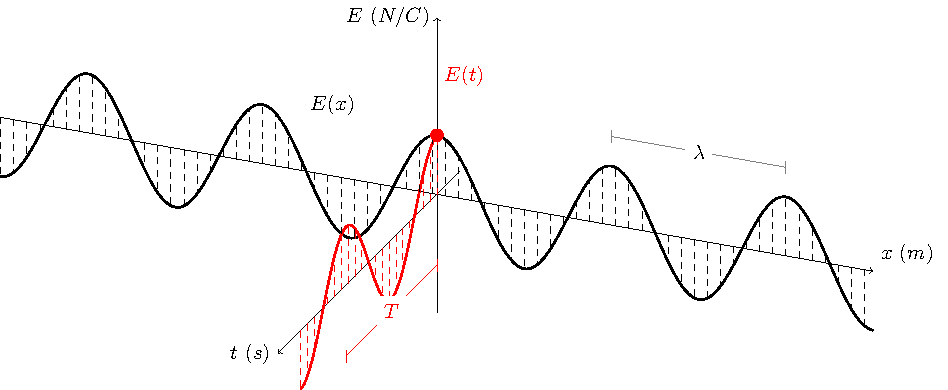
\includegraphics{inputs/module3/module3_tikz_Etrilling_wrapper.pdf}
 %     \caption{Illustratie van een trilling die zich voortplant in de ruimte.}
 %     \label{fig:golflengte_freq}
 % \end{figure}
 % \end{center}

 Als we nu voor het magnetisch veld een gelijkaardige situatie hebben: op elke plaats $x$ zien we een harmonische trilling van het magnetisch veld langs de $z$-as doorheen de tijd en deze trilling plant zich volgens de $x$-as door de ruimte voort.

 Samen vormen beide velden dan een elektromagnetische golf, die zich voorplant, loodrecht op beide velden. 

 \begin{center}
  \tikzsetfigurename{module3_fig_EMgolf}
 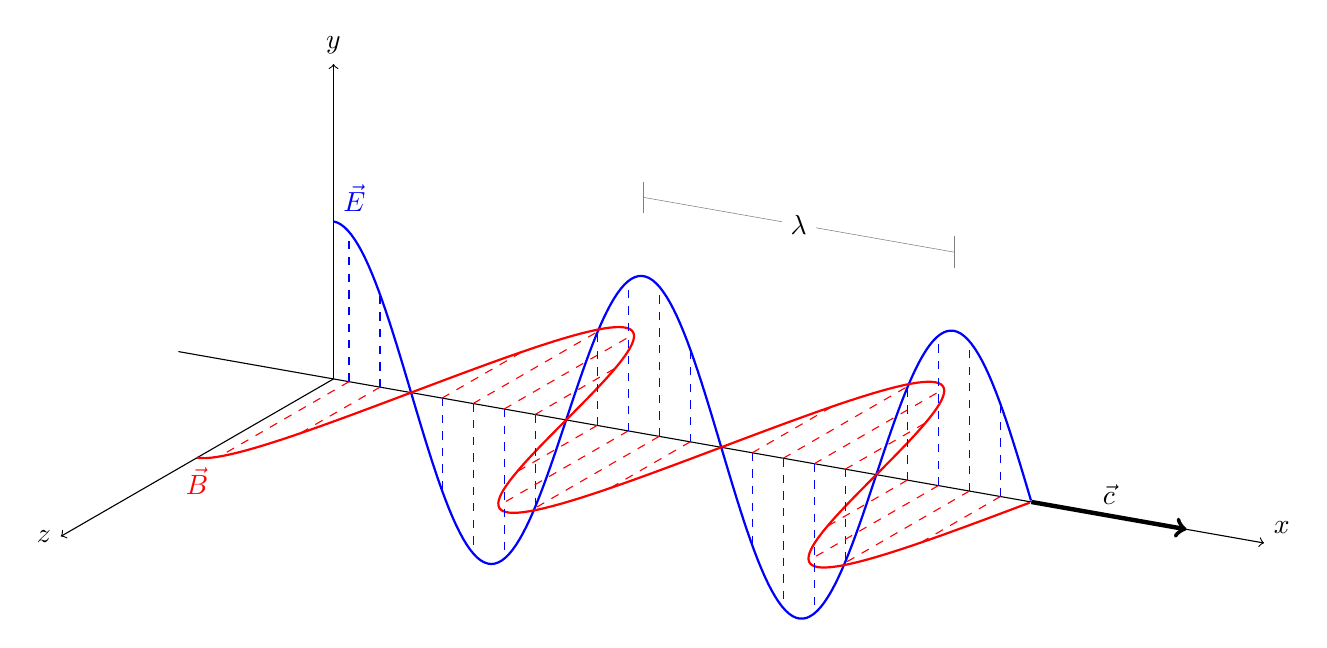
\begin{tikzpicture}[x={(-10:2cm)},y={(90:2cm)},z={(210:2cm)}]
    % Axes
    \draw[->] (-1,0,0) -- (6,0,0) node[above right] {$x$};
    \draw[->] (0,0,0) -- (0,2,0) node[above] {$y$};
    \draw[->] (0,0,0) -- (0,0,2) node[left] {$z$};
    % Propagation
    \draw[->,ultra thick] (4.5,0,0) -- node[above] {$\vec{c}$} (5.5,0,0);
    % Waves
    \draw[thick,blue] plot[domain=0:4.5,samples=200] (\x,{cos(deg(pi*\x))},0);
    \draw[red,thick] plot[domain=0:4.5,samples=200] (\x,0,{cos(deg(pi*\x))});
    % Arrows
    \foreach \x in {0.1,0.3,...,4.4} {
      \draw[-,blue,dashed] (\x,0,0) -- (\x,{cos(deg(pi*\x))},0);
      \draw[-,red,dashed] (\x,0,0) -- (\x,0,{cos(deg(pi*\x))});
    }
    % Labels
    \node[above right,blue] at (0,1,0) {$\vec{E}$};
    \node[below,red] at (0,0,1) {$\vec{B}$};
    
    \draw [help lines] (2, 1.4, 0) -- (2, 1.6, 0);
    \draw [help lines] (4, 1.4, 0) -- (4, 1.6, 0);
    \draw [help lines] (2, 1.5, 0) -- (4, 1.5, 0)
    node [pos =0.5 , fill =white , text = black ]{$ \lambda $};
  \end{tikzpicture}   
 \end{center}
 
  In bovenstaande figuur varieert het elektrisch veld $\vec{E}$ (in blauw) volgens de $y$-as en het magnetisch veld $\vec{B}$ (in rood) volgens de $z$-as. De combinatie van beide oscillaties (loodrecht op elkaar) resulteert in een elektromagnetische golf die zich loodrecht op beide veldvectoren, in dit geval dus volgens de $x$-as, voortplant.
 
  De snelheid waarmee de EM golf voortplant is de lichtsnelheid $c$ ($3 \cdot 10^8$ m/s in vacu\"um). Op de figuur is dit aangeduid als de vector $\vec{c}$ volgens de $x$-as.

 \begin{oef}
 Zijn EM golven transversale of longitudinale golven? Zoek indien nodig op wat bedoeld wordt met transversale en longitudinale golven.
 \end{oef}
 \oplos{EM golven zijn transversale golven, want de trillingen van elektrisch en magnetisch veld staan loodrecht op de voortplantingsrichting.}

 \subsection{Golflengte en frequentie}

 Op Figuur \ref{fig:golflengte_freq} is de golflengte $\lambda$ aangeduid: de afstand waarover de golf zich verplaatst gedurende \'e\'en periode. Of nog: de afstand tussen twee opeenvolgende toppen (of dalen); of de kortste afstand tussen twee punten die in fase trillen.
 We zien ook de periode $T$: de tijd nodig om \'e\'en cyclus te doorlopen. De frequentie is het aantal keer dat een bepaald punt van een golf per seconde op en neer beweegt (met als eenheid $1/s=Hz$).

 In het algemeen geldt dat de voortplantingssnelheid gelijk is aan het product van de \emph{frequentie} met de \emph{golflengte}. EM golven in vacu\"um planten zich voort met de lichtsnelheid in vacu\"um, dus: 

 \begin{equation*}
     \lambda \cdot f = c = 3 \cdot 10^8 \frac{m}{s}
 \end{equation*}

 De lichtsnelheid in een medium, zoals glas of lucht, is lager dan in vacu\"um. De lichtsnelheid $v$ in een medium met brekingsindex $n$ is
 \begin{equation*}
     v = \frac{c}{n}
 \end{equation*}

 De frequentie verandert niet, ongeacht in welk medium de golf voortbeweegt. De golflengte verandert echter wel: de golflengte $\lambda'$ in een medium met brekingsindex $n$ is
 \begin{equation*}
     \lambda' = \frac{v}{f} = \frac{c}{n~f}=\frac{\lambda}{n}.
 \end{equation*}

 De brekingsindex van vacu\"um is $n=1$, terwijl de brekingsindex in lucht gelijk is aan $n=1.0003$.  De voortplantingssnelheid van EM golven in lucht verschilt daarom niet heel veel van de lichtsnelheid van EM golven in vacu\"um. Omdat de lichtsnelheid in alle stoffen lager is dan de lichtsnelheid in het vacu\"um, is de brekingsindex in principe altijd groter dan $1$.

% \begin{oef}
% Schrap wat niet past:
% Indien de brekingsindex van een stof groter is dan $1$, dan is de golflengte van een EM golf in die stof groter/kleiner dan in vacu\"um.
% \end{oef}
% \oplos{Indien de brekingsindex van een stof groter is dan $1$, dan is de golflengte van een EM golf in die stof kleiner dan in vacu\"um.}

 \subsection{Wiskundige voorstelling}

 Op elke plaats in de ruimte waar een elektromagnetische golf aanwezig is, voert het elektrisch en het magnetisch veld een harmonische trilling uit. 

 De uitwijking van het elektrisch veld volgens de $y$-as op plaats $x$ en tijdstip $t$, $E_y(x,t)$, wordt gegeven door:

 \begin{eqnarray*}
     E_y(x,t) &=& E_0 \ cos(\frac{2 \pi}{\lambda} x - 2 \pi f t) \\
     &=& E_0 \ cos(\frac{2 \pi}{\lambda} x - \frac{2 \pi}{T}  t) \\
 \end{eqnarray*}

 De uitwijking van het magnetisch veld volgens de $z$-as op plaats $x$ en tijdstip $t$, $B_z(x,t)$, wordt gegeven door:

 \begin{eqnarray*}
     B_z(x,t) &=& B_0 \ cos(\frac{2 \pi}{\lambda} x - 2 \pi f t) \\
     &=& B_0 \ cos(\frac{2 \pi}{\lambda} x - \frac{2 \pi}{T}  t)
 \end{eqnarray*}
 
 met 
 \begin{itemize}
     \item $E_0$: de amplitude van het elektrisch veld (in $N/C$).
     \item $B_0$: de amplitude van het magnetisch veld (in $T$).
     \item $T$: de periode (in $s$): de tijd nodig om 1 cyclus uit te voeren.
     \item $f=\frac{1}{T}$: de frequentie van de EM golf (in $Hz$): het aantal cycli per seconde.
     \item $\lambda$: de golflengte van de EM golf (in $m$): de afstand waarover de golf zich verplaatst gedurende 1 periode.
 \end{itemize}

 \subsection{Ontstaan van EM golven}
 EM golven kunnen ontstaan op twee manieren:
 \begin{enumerate}
     \item Door ladingen te versnellen \\
     Een elektrische lading, bv. een elektron, die heen en weer beweegt, veroorzaakt een EM golf.
    
     Op deze manier werkt een zendantenne.
     % \gewonefiguur{width=.8\linewidth}{module3/dipoleAntenna}
    
     Een zendantenne bestaat uit twee geleidende staven waartussen een spanningsbron geplaatst is die een wisselspanning opwekt. 
    
     \gewonefiguur{height=5cm}{module3/antenne_AC1}
    
     Beschouw eerst een ogenblik waarop de spanningsbron de bovenste staaf positief laadt en de onderste staaf negatief, zoals in de figuur hierboven. Dan wordt een elektrisch veld (in rood aangeduid op de figuur) opgewekt dat van de bovenste staaf (positief geladen) naar de onderste staaf (negatief geladen) wijst. Doordat de ladingen bewegen, ontstaat ook een magnetisch veld. In elke staaf is de conventionele stroomzin naar boven gericht; volgens de rechterhandregel vinden we dat het magnetisch veld in het blad wijst (in blauw aangeduid op de figuur).
    
     \gewonefiguur{height=5cm}{module3/antenne_AC2}
    
     Op een later moment is de spanning van de wisselspanningsbron van richting veranderd, zoals weergegeven in de figuur hierboven. Nu is de bovenste staaf negatief geladen en de onderste positief, waardoor het elektisch omgekeerd is, en nu van beneden naar boven wijst. Ook de stroomzin is omgekeerd, en het magnetisch veld wijst nu in de omgekeerde zin (uit het blad).
    
     Deze complexe, wisselende interactie tussen elektrische en magnetische velden leidt uiteindelijk tot het ontstaan van EM golven. De frequentie van de EM golf is gelijk aan de frequentie waarmee de spanning opgewekt door de spanningsbron varieert.
    
     \item Ten gevolge van energieprocessen binnen een atoom \\
     Wanneer een atoom overgaat van een hogere energietoestand $E_{hoog}$ naar een lagere energietoestand $E_{laag}$, wordt dat energieverschil als straling uitgezonden. De frequentie van de uitgezonden straling hangt af van het energieverschil tussen beide toestanden:
     \begin{equation}
         f = \frac{E_{hoog}-E_{laag}}{h}
     \end{equation}
     waarbij $h=6.63 \cdot 10^{-34} J \cdot s$ de constante van Planck is.
 \end{enumerate}

 Wanneer we hebben over draadloze communicatie worden de EM golven vooral via de 1e methode opgewekt.

 \subsection{EM spectrum}

 We vermeldden al dat zowel microgolven, zichtbaar licht, r\"ontgenstralen en radiogolven EM golven zijn. EM golven kunnen gecategoriseerd worden a.d.h.v hun frequentie. 

 % Het enige verschil tussen al deze soorten golven is hun golflengte, of equivalent: hun frequentie. 

 \gewonefiguur{width=\linewidth}{module3/EMspectrum}

 \begin{itemize}
     \item Licht \\
     De bekendste vorm van EM straling is licht. Onze ogen zijn gevoelig voor golflengtes tussen 400 nm (violet) en 700 nm (rood). 
    
     Links van licht in het EM frequentiespectrum, met een lagere frequentie bevinden zich de infraroodgolven, microgolven en radiogolven.
    
     \item Infraroodstraling \\
     Infraroodstraling heeft een golflengte tussen $0.7 ~\mu m$ en 1 mm. Infraroodstraling wordt soms ook warmtestraling genoemd omdat we ze als warm ervaren. Warmtecamera's gebaseerd op infraroodstraling kunnen bv. warmteverliezen in een gebouw zichtbaar maken.
     \item Microgolven \\
     De golflengtes van microgolven vari\"eren tussen 30 cm tot 1 mm. Microgolven worden gebruikt bij communicatie met GSM, radars voor vliegtuigen en zoals de naam het zegt om voedsel op te warmen in een microgolfoven. Polaire moleculen (zoals watermoleculen) gaan onder invloed van microgolfstraling trillen. Die trilling zorgt voor opwarming. De gebruikte microgolven worden ook voornamelijk met antennes opgewekt.
     \item Radiogolven \\
     Radiogolven hebben een golflengte van enkele kilometers tot ongeveer 0.3 m. Ze worden vooral gebruikt om radio- en tv-golven te verzenden. Radiogolven worden opgewekt d.m.v. antennes.
    
     Rechts van licht in het EM frequentiespectrum, met een hogere frequentie bevinden zich de ultraviolette straling, r\"ontgenstraling en gammastraling.
    
     \item Ultraviolette (UV) straling \\
     UV-straling heeft een golflengte korter dan zichtbaar licht, tussen 0.6 nm en 400 nm. UV-straling kan de huid verbranden en kanker veroorzaken. De golven worden door atomen en moleculen opgewekt. Zo is de zon een belangrijke bron van UV-straling. De ozonlaag en zonnecr\`eme zijn gelukkig in staat een groot deel van de schadelijke UV-straling te absorberen.
     \item R\"ontgenstraling of X-straling \\
     De golflengte van R\"ontgenstraling varieert van $10^{-4} ~ nm$ tot 10 nm. X-straling wordt ook in atomen opgewekt, door overgang van een hogere naar een lagere energietoestand. X-straling is schadelijk omdat ze ver doordringt in menselijke weefsels en hierbij schade aanricht door atomen te ioniseren of moleculen te dissoci\"eren. De bekendste toepassing van r\"ontgenstraling is medische beeldvorming. 
     \item Gammastraling \\
     Gammstraling hebben een een hele kleine golflengte tussen $10^{-10}$ en $10^{-14}$ m. Ze ontstaan doordat de energie van de deeltjes in de atoomkern wijzigt. Gamma-straling is net als X-straling sterk ioniserend en dus erg schadelijk!
    
 \end{itemize}

 \mybox{
 \subsection*{EM golven in IoT}

 Tot nu toe kwam heel wat theorie i.v.m. EM golven aan bod. Hoog tijd om samen te vatten op welke manier EM golven binnen onze IoT toepassing gebruikt worden.


Er bestaan verschillende draadloze communicatietechnieken. Je kent er vast al een aantal, zoals;
\begin{itemize}
	\item Wifi: communicatie in huis tussen je laptop of smartphone en je wifi-router
	\item 4G: communicatie over grotere afstanden tussen je smartphone en een zendmast
\end{itemize} 

Er bestaan nog een heel aantal andere draadloze communicatietechnieken. Allen maken ze gebruik van EM golven, maar de frequentie die ze hiervoor gebruiken varieert. Wat ook varieert is de afstand waarover communicatie mogelijk is en de hoeveelheid data die kan doorgestuurd worden. 

Bij Wifi kan grote datahoeveelheden (bv gestreamde video) over eerder korte afstanden (bv binnenshuis) gaan doorsturen. Bij 4G kan je wat grotere afstanden overbruggen, maar is de datasnelheid typisch beperkter. Zoals we verderop gaan zien, hangt dit natuurlijk ook af van de aanwezigheid van stoorzenders.

De communicatietechniek die wij gebruiken binnen de IoT toepassing heet LoRa. LoRa is een draadloze communicatietechniek om /emph{beperkte hoeveelheden data over grote afstanden} te verzenden. 

De IoT gateway en sensoren communiceren via EM golven met een frequentie tussen 863 en 870 MHz. 


 \begin{oef}
 \begin{itemize}
     \item Met welke golflengtes komt dit overeen voor voortplanting in de vrije ruimte of in de lucht? 
     \item Over welke soort EM golven spreken we dan?
     \item Hoe worden deze EM golven opgewekt?
 \end{itemize}
 \end{oef}
 \oplos{
 \begin{itemize}
     \item Dit komt overeen met golflengtes tussen 0.345 en 0.348 m.
     \item Dit zijn radiogolven.
     \item Radiogolven worden opgewekt door zendantennes.
 \end{itemize}}
 }
 % \begin{itemize}
 %     \item Itt bedrade communicatie: geen medium
 %     \item Vergelijkbaar met licht = golven
 %     \item Gelijkenissen en verschillen met geluid
 %     \item Frequentie en golflengte
 %     \item Hoe wiskundig voor te stellen?
 %     \item Uitbreiding: ontstaan van EM golven
 % \end{itemize}

\section{Energie en vermogen}

% \begin{itemize}
%     \item Belang van vermogen
%     \item Vermogen van de batterij
%     \item Eventueel uitbreiding elektrochemie/redox
%     \item Vermogen vaak uitgedrukt in dB
%     \item Vermogen afhankelijk van afstand
%     \item Vermogen verliezen: reflectie, attenuatie, diffractie, absorptie (lichtkarakter onderstrepen, invloed van frequentie/golflengte cf. wifi)
%     \item Ontvangen vermogen
% \end{itemize}

Tot nu bespraken we het principe van draadloze signalen en de theorie achter EM golven. In draadloze communicatie is het niet alleen belangrijk te beseffen wat EM straling is, maar ook ervoor te zorgen dat de ontvanger de draadloze signalen met voldoende kwaliteit ontvangt. Je hebt vast wel al gemerkt dat het lastig is je favoriete film via Netflix te streamen teruggetrokken in je slaapkamer, ver weg van het wifi toegangspunt (in de volksmond ook wel router genoemd). Dat komt doordat het wifi-signaal (ook gebaseerd op EM golven) niet voldoende sterk aan je computer aankomt, door de grote afstand tussen je computer en het wifi toegangspunt. Met niet voldoende sterk, bedoelen we dat het vermogen van de EM golf te laag is om nog iets nuttigs mee te kunnen doen. 

In wat volgt spreken we voornamelijk over de voortplanting van radiogolven; die worden het vaakst gebruikt voor draadloze communicatie.

% \subsection{Vermogen van een batterij}

% \subsection{Elektrochemie en redoxreacties}

\subsection{Logaritmisch uitdrukken van vermogen - in deciBel (dB)}
In draadloze communicatie wordt vermogen vaak uitgedrukt in milliwatt, mW.
Omdat vaak heel grote en heel kleine vermogens gebruikt worden, is een handigere eenheid, gebaseerd op logaritmes, de dBm, ingevoerd.
Een vermogen van $1 ~dBm$ komt overeen met $1~mW$. 
Omzetten van een vermogen $P$ in $mW$ naar een vermogen van $x~dBm$, gaat zo:
\begin{equation*}
    x = 10 ~ \log_{10} \frac{P}{1~mW} ~dBm
\end{equation*}

Strikt genomen is $dB$ eenheidsloos: het vermogen in dB wordt immers berekend als een verhouding van twee vermogens, waardoor de eenheid wegvalt. Toch gebruiken we vaak de eenheid $dBm$ i.p.v. gewoon $dB$: de $m$ leert ons immers dat het vermogen dat we bekomen in $dBm$ relatief is t.o.v. een vermogen van $1~mW$ (omdat we delen door $1mW$).

Een vermogen van $100~mW$ komt overeen met 
\begin{equation*}
    10 ~ \log_{10} \frac{100~mW}{1~mW} = 10 \cdot 2 = 20~dBm
\end{equation*}

Hieronder zie je een grafiek die het vermogen $P_{dBm}$ in $dBm$ weergeeft in functie van het vermogen $P$ in $mW$.

\begin{center}
    \begin{tikzpicture}
    %   \draw[->] (-3,0) -- (4.2,0) node[right] {$x$};
    %   \draw[->] (0,-3) -- (0,4.2) node[above] {$y$};
    %   \draw[scale=0.5,domain=-3:3,smooth,variable=\x,blue] plot ({\x},{log10(\x)});
    %   \draw[scale=0.5,domain=-3:3,smooth,variable=\y,red]  plot ({\y*\y},{\y});
    \begin{axis}[no marks,axis lines*=middle,axis line style={shorten >=-10pt,shorten <=-10pt},samples=101,xlabel=$P~(mW)$,ylabel=$P_{dBm}~(dBm)$,label style ={at={(ticklabel cs:1.1)}},ylabel style={rotate=-90}]
    % \addplot {ln(x)};
    \addplot {log10(x)};
    \end{axis}
    \end{tikzpicture}
\end{center}

\mybox{
\subsubsection{De eenheid $dB$}
De eenheid $dB$ wordt vaak gebruikt om geluidssterkte te quantificeren. Geluid is een drukgolf die zich voortplant door de lucht, vanaf een geluidsbron tot aan een ontvanger. 
Die luchtdrukvariaties ten gevolge van geluid kunnen ook over een groot bereik vari\"eren. 

Het menselijk oor is in staat om geluiden te horen tussen een luchtdruk van $p_0 = 0.00002~Pa$ (de geluidsdrempel) en $p=20~Pa$ (de pijngrens). Het is vanzelfsprekend dat de luchtdruk hoger kan zijn dan de pijngrens, maar vervolgens pijn aan de oren veroorzaakt. 
Het luchtdrukbereik tussen de gehoorgrens en de pijngrens dat mensen kunnen waarnemen is ongelooflijk groot ($10^{6}$). Wellicht is hierdoor het volume dat wij ervaren niet recht evenredig met de luchtdruk. Om een geluid te ervaren dat dubbel zo hard klinkt, moet de luchtdruk ongeveer met een factor $20$ toenemen. Daarom wordt een nieuwe grootheid ingevoerd: de \emph{geluidssterkte} met als eenheid de decibel, afgekort als $dB$.

De geluidssterkte $L_p$ wordt bepaald als het logaritme van de verhouding van de luchtdruk $p$ van het geluid ten opzichte van de gehoorgrens $p_0 ~ = ~ 0.00002~Pa$: 

\begin{equation*}\label{eq:dbp}
L_p = 20 \cdot log \bigg(\frac{p}{p_0}\bigg)
\end{equation*}
\vspace{1mm}
}

Hier zie je opnieuw duidelijk dat de $dB$ een dimensieloze eenheid is, doordat de verhouding van twee grootheden genomen wordt.

We geven nog enkele vaakgebruikte waarden mee: een toename in vermogen van $10~dB(m)$ komt overeen met een vertienvoudiging van het vermogen. Een toename van $3~dB(m)$ komt ongeveer overeen met een verdubbeling. We gebruiken hier over de eenheid $dB(m)$, omdat deze verbanden ($+10~dB$ is maal 10 en $+3~dB$ is maal 3) gelden voor elke grootheid uitgedrukt in $dB$, of het nu om een vermogen of om een geluidssterkte of nog een andere grootheid gaat.

\begin{voorbeeld}
We geven een voorbeeld: als we een vermogen $P_1$ van $7~dBm$ verhogen met $3~dBm$, bekomen we een vermogen $P_2$ van $10~dBm$. Een vermogen van $7~dBm$ komt ongeveer overeen met $5~mW$; een vermogen van $10~dBm$ komt ongeveer overeen met $10~mW$. Het vermogen $P_2$ is dus inderdaad ongeveer het dubbele van het vermogen $P_1$.
\end{voorbeeld}

We rekenen dit even door. Een vermogen $P_2 \text{ (in dBm)} = P_1 \text{ (in dBm)} + 3~dBm$ komt overeen met het dubbele van $P_1$. Immers: 

\begin{eqnarray*}
    P_2~(dBm)&=& 10*\log_{10} P_1 + 3~dBm \\
    &=& 10*\log_{10} P_1 + 10*\log_{10} 10^{\frac{3}{10}} \\
    &=& 10*\log_{10} P_1 \cdot 10^{0.3}\\
    &=& 10 \log_{10} 2 P_1 \\
    P_2 &=& 2 P_1
\end{eqnarray*}

\begin{oef}
Hoeveel $dBm$ is 
\begin{itemize}
    \item 10 mW
    \item 250 mW
    \item 100 W
\end{itemize}
\end{oef}
\oplos{
\begin{itemize}
    \item $10 ~mW = 10 \cdot 1 ~dBm = 10~dBm$
    \item $250 ~mW = 10 \cdot \log_{10} 250 ~dBm = 24~dBm$
    \item $100 ~W = 10 \cdot \log_{10} \frac{100000}{1} ~dBm = 50~dBm$
\end{itemize}
}

\begin{oef}
Hoe bereken je het vermogen $P$ in $mW$ als het vermogen $x$ in $dBm$ gegeven is?
\end{oef}
\oplos{\begin{equation*}
    P = 10^{\frac{x}{10}} ~ mW
\end{equation*}}

\subsection{Demping: het ontvangen vermogen hangt af van de afstand tot de zendantenne}

We bekijken eerst een ideale situatie: de vrije ruimte. We bedoelen hiermee letterlijk de ruimte: een vaccu\"um waarin geen objecten voorkomen.

In die ideale situatie wordt het ontvangen vermogen $P_o$ (in $W$) bij een draadloze verbinding gegeven door de radiovergelijking:

\begin{equation}
    P_o = G_z ~ G_o ~ (\frac{\lambda}{4 \pi d})^2 ~P_z
    \label{eq:radiovgl}
\end{equation}

met
\begin{itemize}
    \item $P_z$ (in $W$) het uitgezonden vermogen, 
    \item $G_z$ en $G_o$ (zonder eenheid) respectievelijk de winst van de zend- en de ontvangantenne, 
    \item $\lambda$ (in $m$) de golflengte van de radiogolf, en 
    \item $d$ (in $m$) de afstand tussen de zender en de ontvanger.  
\end{itemize}
De antennewinsten $G_z$ en $G_o$ zijn getallen die aangeven hoe goed de antennes een EM golf kunnen uitsturen/ontvangen. Merk de sterke afhankelijkheid van de afstand op: de verzwakking op een radioverbinding neemt toe de afstand in het kwadraat!

De theoretische formule voor vrije ruimte propagatie mag enkel gebruikt worden voor radioverbindingen tussen twee antennes die zich op voldoende afstand bevinden van het aardoppervlak en van andere reflecterende en absorberende objecten. In dat geval bestaat het ontvangen signaal quasi enkel uit radiogolven die rechtstreeks van zender naar ontvanger bewegen. Bovendien moet de absorptie op dit rechtstreekse pad verwaarloosbaar zijn.

Een duidelijk voorbeeld waar de vrije ruimte benadering toepasbaar is, is een radioverbinding tussen satellieten in de ruimte.

\begin{oef}
\begin{itemize}
    \item Wat is het ontvangen vermogen in Watt als een antenne met een vermogen van $5 \cdot 10^{-2} ~W$ een EM signaal met een frequentie van $2.4~GHz$ over een afstand van $5~m$ verzendt, met antennewinsten van $G_z=G_o=1$?
    \item Wat is het vermogen in $dBm$?
\end{itemize}
\end{oef}
\oplos{TODO}

\begin{oef}
Vorm de radiovergelijking (vgl \ref{eq:radiovgl}) om voor vermogens uitgedrukt in $dBm$ (i.p.v. in $W$).
\end{oef}
\oplos{$P_{o,dBm} = G_{z,dBm} + G_{o,dBm} + 20 \cdot \log_{10} (\frac{\lambda}{4\pi d}) + P_{z,dBm}$}

\subsection{Voortplanting van EM golven op aarde}

Op aarde is de situatie een stuk complexer dan in de vrije ruimte, en dienen we een onderscheid te maken naar de frequentie van de radiogolven om de voortplanting te kunnen karakteriseren. Of voor een radiogolf reflecterende oppervlakken \textquotedblleft ver\textquotedblright \ en of obstakels \textquotedblleft groot\textquotedblright \ zijn, hangt immers af van de golflengte, en dus de frequentie, van de radiogolven.

\subsubsection{Blokkering}
Blokkering van EM golven door grote obstakels is een extreme vorm van verzwakking. Bij grote obstakels geldt: hoe hoger de frequentie van een signaal, hoe kleiner de golflengte, hoe vergelijkbaarder met licht. Voor signalen met een kleine golflengte en dus met een hoge frequentie, kunnen zelfs \textquotedblleft kleine\textquotedblright \ obstakels (zoals een schrift, een verkeersbord enz.) het signaal al blokkeren. Bij signalen met een grote golflengte daarentegen zijn grote obstakels nodig om het signaal te blokkeren. Daarom worden radiogolven vaak gebruikt voor draadloze communicatie: die golven hebben een grote golflengte en worden dus slechts door grotere objecten geblokkeerd.

\subsubsection{Reflectie}

Als een obstakel groot is t.o.v. de golflengte van het signaal, dan wordt het signaal weerkaatst. Dit noemen we reflectie. Dit verschijnsel hebben jullie zeker al geobserveerd met (laser)licht in de tweede graad. Bij elke reflectie wordt het signaal/het licht ook een beetje verzwakt: we zeggen dat de \emph{gereflecteerde golf minder vermogen heeft}.

\begin{center}
\begin{tikzpicture}
  \draw[gray,fill=gray,path fading=south] (0,0) rectangle +(5,-2);% sample
    \begin{scope}[decoration={snake,amplitude=.4mm,
        segment length=2mm,post length=1mm}]
      \draw[decorate,blue,-<]  (2.5,0) -- ++(135:3);% invallend
      \draw[decorate,orange,->] (2.5,0) -- ++(45:3);% gereflecteerd
    \end{scope}
  %labels
  \draw (0,-2) node[above right] {\footnotesize Medium ($n$)};
  \draw (2.5,0) ++(45:3) node[right] {\footnotesize Gereflecteerde golf};
  \draw (2.5,0) ++(135:3) node[left] {\footnotesize Invallende golf};
\end{tikzpicture}
\end{center}

Reflectie kan zowel constructief als destructief werken.
\begin{itemize}
    \item Constructief \\
    
    We spreken van een \emph{zichtlijn} als er een signaal ononderbroken kan voortplanten op een rechte lijn tussen zender en ontvanger.
    O.a. wanneer er geen zichtlijn aanwezig is tussen zender en ontvanger, kan reflectie een positief effect hebben op de signaalvoortplanting. 
    % Een zichtlijn is een rechte lijn tussen zender en ontvanger waarlangs het draadloos signaal zich voortplant.
    
    \gewonefiguur{width=\linewidth}{module3/reflectie-constructief-onderbroken-zichtlijn}
    
    Reflectie kan ervoor zorgen dat het signaal toch bij de ontvanger kan aankomen, ook wanneer er geen zichtlijn tussen zender en ontvanger is, zoals in de figuur hierboven. De zender is de IoTree node, die aan de boom hangt. De gateway staat op de top van het appartementsgebouw. Door het huis is er geen zichtlijn tussen Iotree node en gateway. Gelukkig zorgt de geparkeerde vrachtwagen ervoor dat de gateway toch het IoTree signaal kan ontvangen!
    
    Er is nog een geval wanneer reflectie constructief werkt. Stel dat er bij de ontvanger twee signalen aankomen: (1) het rechtstreekse signaal via de zichtlijn, en (2) een gereflecteerd signaal doordat het uitgezonden signaal reflecteert op bv. het aardoppervlak. Het gereflecteerde signaal zal iets later bij de ontvanger aankomen dan het rechtstreekse signaal, omdat het een langere weg moet afleggen. We zeggen dat er een \emph{faseverschil} tussen beide signalen is. Het faseverschil is afhankelijk van de golflengte van het draadloos signaal en van het weglengteverschil tussen het gereflecteerde en het rechtstreekse signaal. Beide signalen worden bij de ontvanger gesommeerd. Hoe groot het gesommeerde signaal is, hangt af van het faseverschil.
    
    \gewonefiguur{width=\linewidth}{module3/reflectie-constructief}
    
    In het ene extreme geval is het faseverschil een even veelvoud van 180 graden. In dat geval zijn beide ontvangen signalen \emph{in fase} en versterken beide signalen elkaar. Het ontvangen signaal is dan dubbel zo sterk als het oorspronkelijk verzonden signaal. Dit noemen we constructieve interferentie.
    
    \item Destructief \\
    Reflectie kan er echter ook voor zorgen dat het signaal zeer verzwakt bij de ontvanger aankomt. 
    
    \gewonefiguur{width=\linewidth}{module3/reflectie-destructief}
    
    Neem opnieuw het geval wanneer er bij de ontvanger twee signalen aankomen: (1) het rechtstreekse signaal via de zichtlijn, en (2) een gereflecteerd signaal doordat het uitgezonden signaal reflecteert op bv. het aardoppervlak. We hebben het ene extreme geval waarbij beide signalen elkaar versterken al besproken.
    
    In het andere extreme geval is het faseverschil een oneven veelvoud van 180 graden. In dat geval zijn beide ontvangen signalen \emph{in tegenfase} en doven beide signalen elkaar uit. Er wordt dan helemaal geen signaal ontvangen bij de ontvanger. Dit noemen we destructieve interferentie.
    \item Mengvorm \\
%    {\color{red} TODO invoegen figuur illustratie weglengteverschil}
    In de realiteit is het weinig waarschijnlijk dat het rechtstreekse en het gereflecteerde signaal elkaar volledig gaan uitdoven. Dan krijgen we mengvormen: de ene keer versterken beide signalen elkaar (een beetje), de andere keer verzwakken ze elkaar (een beetje). Het precieze effect is moeilijk voor elke situatie op voorhand te voorspellen.
\end{itemize}

We kunnen dit effect ook wiskundig beredeneren. Veronderstel dat een zender een sinusoïdaal EM signaal $z(t)$ uitstuurt. Bij de ontvanger komt het signaal rechtstreeks, via een rechte lijn tussen zender en ontvanger, aan. Dit is het signaal $z(t)$. Er is echter ook een gereflecteerd EM signaal dat de ontvanger bereikt: het signaal $r(t)$. Dit zie je schematisch weergegeven in de bovenstaande figuren en ook op onderstaande figuur. 

\begin{center}
    \begin{tikzpicture}
        \begin{axis}[no marks,axis lines=center,samples=101,xlabel=$t$,ylabel=$z(t)$,label style ={at={(ticklabel cs:1.1)}}]
        % \begin{axis}[no marks,axis lines=center,samples=101]
        % \addplot {ln(x)};
        \addplot {sin(deg(x))};
        \end{axis}
    \end{tikzpicture}
    
    \begin{tikzpicture}
        \begin{axis}[no marks,axis lines=center,samples=101,xlabel=$t$,ylabel=$r(t)$,label style ={at={(ticklabel cs:1.1)}}]
        % \begin{axis}[no marks,axis lines=center,samples=101]
        % \addplot {ln(x)};
        \addplot {sin(deg(x+1.5))};
        % \node[]
        \end{axis}
    \end{tikzpicture}
\end{center}

Bij de ontvanger is het totale ontvangen signaal $o(t)$ de som van het rechtstreekse $z(t)$ en het gereflecteerde EM signaal $r(t)$:

\begin{eqnarray*}
o(t) &=& z(t) + r(t) \\
&=& A~\sin(2 \pi f t) + A~\sin(2 \pi f t + \delta) \\
&=& 2A ~ \cos(\frac{\delta}{2}) ~ \sin(2 \pi f t + \frac{\delta}{2}) 
\end{eqnarray*}

Omdat het signaal $r(t)$ een langere weg heeft afgelegd dan het signaal $z(t)$, komt dit signaal met een andere fase bij de ontvanger aan. We zeggen dat er een faseverschil is tussen beide signalen. Dit faseverschil duiden we aan met het symbool $\delta$. De waarde van het faseverschil hangt af van het weglengteverschil (= het verschil in afstand dat beide signalen moesten afleggen) en van de golflengte van de EM signalen.

Door de formule van Simpson toe te passen zien we dat er aan de ontvanger een EM golf waargenomen wordt met als amplitude $2A ~ \cos(\frac{\delta}{2})$. Hieronder zie je de resulterende amplitude voor verschillende waarden van $\delta$.

\begin{tabel}{}
\begin{tabular}[h]{l|l} 
$\delta$ & $2A ~ \cos(\frac{\delta}{2})$ \\
\hline
$0^{\circ}$ & $2A$ \\
$90^{\circ}$ & $2A \ cdot \frac{\sqrt{2}}{2} = \sqrt{2} A$ \\
$180^{\circ}$ & $0$ \\
$270^{\circ}$ & $2A \ cdot \frac{\sqrt{2}}{2} = \sqrt{2} A$\\
\end{tabular}
\end{tabel}

Wanneer het weglengteverschil zodanig is dat het faseverschil tussen het rechtstreekse en het gereflecteerde signaal $180^{\circ}$ bedraagt, wordt aan de ontvanger helemaal geen signaal waargenomen: het rechtstreekse en het gereflecteerde signaal heffen elkaar volledig op. Volledige versterking krijgen we wanneer het weglengteverschil tussen het rechtstreekse en het gereflecteerde signaal resulteert in een faseverschil van een veelvoud van $360^{\circ}$. Alle faseverschillen daartussen resulteren in een amplitude tussen $0$ en $2A$.

In het geval waarbij bij de ontvanger zowel een rechtstreeks signaal als (\'e\'en of meerdere) gereflecteerd(e) signa(a)l(en) aankomen hebben we in feite te maken met een echo-verschijnsel. Men noemt men dit een multi-pad situatie. 

% XXXXXXXXXX toont een voorbeeld van multi-pad propagatie bij GSM-communicatie in een stedelijke omgeving, waarbij er vaak zelfs geen rechtstreekse component meer ontvangen wordt.

% Welk effect de multi-pad propagatie heeft op de doorgezonden informatie, hangt voornamelijk af van het relatieve weglengteverschil t.o.v. de golflengte die de verschillende signalen hebben afgelegd. De twee extreme gevallen treden op wanneer het weglengteverschil een geheel aantal halve golflengtes bedraagt: bij een even aantal versterken de golven elkaar maximaal, terwijl ze elkaar bij een oneven aantal halve golflengtes gaan uitdoven (zie XXXXXXXXXXXXXX). Deze verschijnselen noemt men respectievelijk positieve en negatieve interferentie.

%{\color{red} TODO oefening!}

\subsubsection{Breking/refractie}
Breking is het verschijnsel dat EM stralen van richting veranderen als ze van het ene medium in het andere terechtkomen. De breking van licht hebben jullie ook in de tweede graad leren kennen. Dit effect treedt op omdat de snelheid van EM golven afhangt van het medium waar ze doorheen bewegen.

% \begin{center}
% \begin{tikzpicture}
%   \draw[gray,fill=gray,path fading=south] (0,0) rectangle +(5,-2);% sample
%     \begin{scope}[decoration={snake,amplitude=.4mm,
%         segment length=2mm,post length=1mm}]
%       \draw[decorate,blue,-<]  (2.5,0) -- ++(135:3);% invallend
%       \draw[decorate,orange,->] (2.5,0) -- ++(45:3);% gereflecteerd
%         \draw[decorate,red,->] (2.5,0) -- ++(290:3);% gebroken
%     \end{scope}
%   %labels
%   \draw (0,2) node[above right] {\footnotesize Medium 1 ($n_1$)};
%   \draw (0,-2) node[above right] {\footnotesize Medium 2 ($n_2$)};
%   \draw (2.5,0) ++(45:3) node[right] {\footnotesize Gereflecteerde golf};
%   \draw (2.5,0) ++(135:3) node[left] {\footnotesize Invallende golf};
%   \draw (2.5,0) ++(290:-3) node[left] {\footnotesize Gebroken golf};
% \end{tikzpicture}
% \end{center}

De brekingshoek $\theta_2$ kan je bepalen met de wet van Snellius, als je de invalshoek $\theta_1$ en de brekingsindices in medium 1 $n_1$ en medium 2 $n_2$ kent:
\begin{equation*}
    \frac{\sin(\theta_1)}{\sin(\theta_2)} = \frac{n_1}{n_2}
\end{equation*}

De vorige drie verschijnselen (blokkering, reflectie en breking) treden vooral op wanneer de obstakels groot zijn in vergelijking met de golflengte van de EM golven. Deze drie verschijnselen hebben jullie voornamelijk in het dagelijkse leven en in de tweede graad kunnen waarnemen. Ze illustreren vooral het deeltjeskarakter van licht.

De volgende drie verschijnselen treden eerder op bij obstakels die van dezelfde grootteorde of kleiner zijn dan de golflengte van de EM golven. Ze illustreren het golfkarakter van licht.

\subsubsection{Attenuatie en absorptie}

Naarmate de golflengte van een radiogolf korter wordt, neemt de invloed van \textquotedblleft kleine\textquotedblright \ deeltjes in de atmosfeer toe. Deze deeltjes kunnen zowel vloeibaar, vast, als gasvormig zijn. Zo zien we de verzwakking op draadloze verbindingen bij zware regenval drastisch toenemen bij hoge frequenties (GHz-gebied), en ook sneeuw en mist kunnen onwelkome spelbrekers zijn. Resonantiepieken in de absorptie van bepaalde gassen die aanwezig zijn in de lucht, kunnen de communicatie bij specifieke frequenties enorm bemoeilijken. Het meest actuele voorbeeld hiervoor is wellicht de absorptiepiek van zuurstof bij 60 GHz, die maakt dat bij deze frequenties zelfs propagatie in de lucht zonder enig ander obstakel slechts een zeer beperkte reikwijdte heeft.

\subsubsection{Verstrooiing (Engels: scattering)}

Als de golflengte van EM golven gelijkaardig of groter is dan een object, kunnen de EM golven verstrooid raken. Een invallend signaal wordt dan verstrooid in verschillende zwakkere signalen die zich in verschillende richtingen voortplanten. 

\gewonefiguur{width=\linewidth}{module3/scattering}

Bij draadloze communicatie hebben we te maken met EM golven met een veel grotere golflengte, die reeds bij veel grotere objecten (in de grootteorde van enkele tientallen cm) kunnen verstrooid worden.

\subsubsection{Diffractie}

Diffractie is het afbuigen van een golf langs een obstakel. Op school wordt dit gedemonstreerd met laserlicht dat verstrooid wordt rondom een zeer kleine opening.  

Diffractie is sterk gerelateerd aan verstrooiing. In beide gevallen worden EM golven na contact met een obstakel verzwakt in verschillende richtingen voortgeplant. In beide gevallen leidt dit tot een patroon met uiteenlopende signaalsterkte. De gebruiker kan een versterkt of een verzwakt signaal waarnemen, afhankelijk van zijn exacte positie.

\begin{oef}
Maak een overzicht van de verschijnselen die optreden bij EM golven op aarde. 
Gebruik hiervoor een tabel met volgende opbouw:
\begin{itemize}
    \item Verschijnsel: naam en beschrijving. Maak eventueel een figuur ter verduidelijking.
    \item Grootte van de objecten waarbij dit verschijnsel optreedt. Druk de grootte op t.o.v. de golflengte van de EM straling: groot/klein t.o.v. $\lambda$.
    \item Gevolg voor communicatie met EM golven: loopt de communicatie makkelijker of net moeilijker? Of hangt dit net af van de specifieke situatie?
\end{itemize}
\end{oef}

\subsection{Ruis}
Succesvolle communicatie hangt af van hoe goed de ontvanger de informatie kan halen uit de doorgestuurde signalen. Zelfs in het geval er nauwelijks vervorming van de radiogolven optreedt op het kanaal, dan nog is een perfecte ontvangst nooit mogelijk omwille van de ruis die onvermijdelijk op de signalen gesuperponeerd wordt. De term ruis wordt gedefinieerd als alle ongewenste signalen die zich bij de eigenlijke informatie voegen. Men kan voor de meeste communicatiesystemen stellen dat de verhouding van het signaalvermogen tot het ruisvermogen bepalend is voor de kwaliteit van een verbinding. Ruis kan zowel van natuurlijke als van menselijke oorsprong zijn.

\gewonefiguur{width=\linewidth}{module3/additieveRuis}

\subsubsection{Ruis van natuurlijke oorsprong}

Een belangrijke natuurlijke ruisbron is de thermische ruis. Thermische ruis ontstaat doordat alle elektronen onder invloed van de temperatuur een zekere beweeglijkheid hebben. Het is bijgevolg fysisch onmogelijk om een volledig ruisvrij elektrisch systeem te bouwen, al kan men de thermische ruis wel proberen te minimaliseren. Omdat de thermische bewegingen van de elektronen willekeurig zijn van aard, is ook de ruis een random signaal. Thermische ruis manifesteert zich bovendien ongeveer even sterk bij alle frequenties, en heeft een dichtheid $n_0$ die temperatuursafhankelijk is:

\begin{equation*}
    n_0 = k~T ~ [W/Hz]
\end{equation*}

waarbij $k$ de constante van Boltzmann is ($k =1,38.10^{-23}~J/K$ ) en $T$ de temperatuur uitgedrukt in graden Kelvin.

TODO oefening: hoe hoger de temperatuur, hoe meer/minder ruis

Andere natuurlijke ruisbronnen die van belang zijn voor draadloze verbindingen zijn o.a. storingen in de atmosfeer en straling die van de zon en andere elementen uit onze eigen melkweg en daarbuiten komen. Meestal hebben deze ruisbronnen een veel kleiner effect dan de thermische ruis, maar soms kunnen ze de communicatie toch ernstig storen, zoals men bijvoorbeeld kan vaststellen wanneer men tijdens een lokaal onweer naar de radio luistert.

\subsubsection{Ruis van menselijke oorsprong}

De activiteit van de mens veroorzaakt ook heel wat ruis in de ether.

Omwille van de hinder die ze veroorzaken voor de draadloze communicatie, wordt de maximale straling die industri\"ele machines in bepaalde frequentiebanden mogen afgeven, bij wet vastgelegd. Ook binnenshuis kan bijvoorbeeld een PC, die nogal wat hoogfrequente signalen genereert, voor heel wat extra storing op de radio-ontvangst zorgen.

Vaak ontvangt men bij draadloze verbindingen stoorsignalen die veroorzaakt worden door andere zenders die op dezelfde frequenties communiceren of op zijn minst ruis genereren in die band waar het gewenste signaal doorgestuurd wordt. De overheid tracht dit door de regularisatie van het frequentiespectrum te voorkomen. Dit specifiek soort ruis noemt men interferentie. Interferentie vormt een steeds groter probleem door de steeds toenemende draadloze communicatie.

\subsubsection{Signaal-ruisverhouding $SNR$ (Engels: signal-to-noise-ratio)}

Dit is een maat die uitdrukt hoe groot het signaalvermogen is in vergelijking met het ruisvermogen. 

\begin{equation*}
    SNR = \frac{S}{N}
\end{equation*}
Met: 
\begin{itemize}
    \item S is het signaalvermogen, uitgedrukt in $W$
    \item N is het ruisvermogen, eveneens uitgedrukt $W$
\end{itemize}

De signaalruisverhouding, of de SNR, wordt vaak in dB uitgedrukt:

\begin{equation*}
    SNR_{dB} = 10 ~ \log_{10} \left( \frac{S}{N} \right)
\end{equation*}

Hieronder zie je enkele figuren van een ruizig signaal met verschillende signaalruisverhoudingen.

\gewonefiguur{width=\linewidth}{module3/ruisVerschillendeSNRs}

\subsection{Signaalvoortplanting voorspellen?}

Bovengenoemde effecten, demping, absorptie en attenuatie, reflectie, breking, verstrooiing en diffractie, ruis en interferentie, doen zich allen tegelijk voor en zijn frequentie-afhankelijk. Het is zeer lastig om de precieze signaalsterkte in elke plaats in de (stads)omgeving te voorspellen. Bijvoorbeeld bij GSM-communicatie voeren GSM-operatoren daarom metingen uit om het bereik van hun zend- en ontvangstantennes in kaart te brengen en indien nodig gaten in de dekking op te vullen. 

Uiteraard vari\"eren veel van deze effecten ook in de tijd: denk aan een vrachtwagen die via reflectie communicatie tussen een GSM en zendmast mogelijk maakt. Wanneer deze vrachtwagen zich verplaatst, valt ook de reflectie weg en zal het draadloze GSM-signaal via een ander pad de zendmast moeten bereiken.

\mybox{
\subsection*{Signaalvoortplanting in IoT toepassingen}

Tot nu toe kwam heel wat theorie i.v.m. vermogenverliezen bij draadloze communicatie aan bod. Hoog tijd om samen te vatten hoe dit alles relateerd met IoTree.

In IoT toepassingen wordt informatie van de sensoren doorgestuurd naar de gateway. 

\begin{oef}
\begin{itemize}
    \item Welk soort vermogenverliezen verwacht je in een stedelijke omgeving? En in een binnenomgeving?
    \item Wat is het ontvangen vermogen voor satellietcommunicatie met 
    \begin{itemize}
    \item een zendvermogen van 200 dBm 
    \item een zend- en ontvangstantennewinst van 1
    \item een afstand van 1 km tussen zender en ontvanger?
    \end{itemize}
\end{itemize}
\end{oef}
\oplos{
\begin{itemize}
    \item Vermogenverliezen door reflectie, absorptie en diffractie.
    \item {\color{red} TODO uitrekenen}
\end{itemize}
}

De situatie is vaak nog wat ingewikkelder dan wat we tot nu toe bekeken hebben. Wij hebben - bijvoorbeeld bij reflectie - steeds signalen met 1 frequentie, bv een sinus, bekeken. Bovendien zijn die signalen periodisch. In de realiteit bevatten vangt een gateway signalen op van meerdere gebruikers en bevatten die signalen vaak meerdere frequenties en zijn ze niet periodisch. Dit leidt tot nog sterkere verstoring van het doorgestuurde signaal en zorgt ervoor dat er hele goede communicatie-afspraken nodig zijn om toch de doorgestuurde data te kunnen reconstrueren! 

}

\section{Kanaalcapaciteit}

De maximale capaciteit van een kanaal is de maximale hoeveelheid informatie die over het kanaal verzonden kan worden per tijdseenheid. Informatie (bv. spraaksignalen, video, temperatuurswaarden, ...) worden op een computer als een binair getal, bestaande uit eentjes en nulletjes, opgeslagen. Onafhankelijk van het type informatie (video, geluid, getallen, tekst) wordt de hoeveelheid informatie gegeven door het aantal eentjes en nulletjes (bits) nodig om die informatie te vatten. 

Een foto is typisch een grote 2MB groot. Per seconde video heb je al 400MB nodig. Andere sensoren kunnen een veel beperktere geheugencapaciteit vereisen, bv. slechts 2 bytes voor een temperatuursmeting.

De hoeveelheid informatie die gedurende een tijdseenheid over een kanaal gestuurd kan worden wordt uitgedrukt in bits/s: hoeveel bits kan je per tijdseenheid/seconde over het kanaal verzenden?

De kanaalcapaciteit $C$ (eenheid: bits/s) wordt gegeven door:

\begin{equation*}
    C = B ~ \log_2 (1+\frac{S}{N})
\end{equation*}

hierbij is 
\begin{itemize}
    \item B: de bandbreedte van het kanaal (eenheid: Hz)
    \item $\frac{S}{N}$: de signaal-ruisverhouding van het kanaal (zonder eenheid).
\end{itemize}

Let op: de kanaalcapaciteit is de maximaal haalbare hoeveelheid informatie die over een kanaal verzonden kan worden! Het is een fysisch optimum. Om deze datasnelheid ook werkelijk te bereiken, moeten slimme trucjes toegepast worden. Zo bepaalt de informatieoverdrachttechniek (zie volgende paragraaf) in grote mate de bereikte datasnelheid.

\begin{voorbeeld}
We berekenen de kanaalcapaciteit voor een signaalruis-verhouding van $26~dB$ en een bandbreedte van $4~kHz$.

\begin{itemize}
    \item Eerst moeten we de signaalruis-verhouding \textquotedblleft lineair \textquotedblright uitdrukken: we moeten de $dB$-waarde omzetten naar een gewone lineaire verhouding.
    
    \begin{eqnarray*}
        \frac{S}{N} &=& 26~dB \\
        &=& 10^{26/10} \\
        &=& 398
    \end{eqnarray*}
    
    \item Als we de lineaire signaalruis-verhouding kennen, kunnen we formule voor de kanaalcapaciteit toepassen:
    
    \begin{eqnarray*}
    C &=& B ~ \log_2(1+\frac{S}{N}) \\
    &=& 4000 ~ \log_2(1+398) \\
    &=& 4000 ~ \log_2(399) \\
    &=& 34.6 ~\text{kbit/s}
    \end{eqnarray*}
\end{itemize}
\end{voorbeeld}

\begin{voorbeeld}
Als de maximale datasnelheid voor een applicatie 100 kbit/s moet zijn en de bandbreedte van het kanaal is 2 MHz, bereken dan de nodige signaalruis-verhouding.

We starten vanuit de formule voor kanaalcapaciteit en berekenen hieruit de minimale signaalruis-verhouding:

    \begin{eqnarray*}
    C &=& B ~ \log_2(1+\frac{S}{N}) \\
    \num{100 000} &=& \num{2000000} ~ \log_2(1+\frac{S}{N}) \\
    100 &=& 2000 ~ \log_2(1+\frac{S}{N}) \\
    \\
    \log_2(1+\frac{S}{N}) &=& \frac{1}{20} \\
    \\
    \frac{S}{N} &=& 2^{\frac{1}{20}}-1 \\
    &=& 0.035 \\
    &=& -14.5~dB
    \end{eqnarray*}
    
Hieruit volgt dat het mogelijk is signalen te verzenden die zwakker zijn (minder vermogen hebben) dan de ruis uit de omgeving. De signaalruisverhouding is immers kleiner dan 1, of equivalent: kleiner dan $0~dB$. Hiervoor moeten wel speciale draadloze informatieoverdrachttechnieken gebruikt worden. Die informatieoverdrachttechnieken worden in de volgende paragraaf besproken.
\end{voorbeeld}

\section{Hoe informatie overdragen?}

De zender moet de informatie omzetten in een vorm die geschikt is voor de draadloze transmissie via radiogolven. 
Daartoe worden de signalen gemoduleerd op een draaggolf.

Tijdens het modulatie-proces wordt een parameter van een EM golf gevarieerd. Die EM golf is vaak een hoogfrequente (grootte-orde MHz) sinuso\"idale radiogolf.
Modulatie is het combineren van een laagfrequent informatiesignaal met een zo'n hoogfrequente draaggolf. Daardoor ontstaat een signaal met een frequentieband rondom de frequentie van de draaggolf.

Stel dat een radio- of televisiesignaal direct zonder draaggolf draadloos wordt uitgezonden. Het audiosignaal dat door een microfoon wordt opgewekt, en frequenties onder 20 kHz bevat, zou dus dan met die frequenties worden uitgezonden. Er zou dan maar één zender tegelijk in bedrijf kunnen zijn, maar het grootste probleem is dat dergelijke frequenties zich niet goed voortplanten door de atmosfeer.

Dit probleem wordt opgelost door het bronsignaal met een draaggolf met een veel hogere frequentie over te brengen. Met een modulator wordt het signaal gesuperponeerd op een sinusvormige draaggolf, waaruit later door demodulatie het oorspronkelijke signaal weer kan worden teruggewonnen. 

Typische voorbeelden van klassieke analoge modulatietechnieken zijn AM (amplitude modulatie) en FM (frequentie modulatie). 
Door verschillende signalen op draaggolven te moduleren met frequenties die ver genoeg van elkaar liggen, kan men bovendien tegelijkertijd meerdere gebruikers op hetzelfde kanaal laten communiceren. 
Dit is het mechanisme van meervoudige toegang in het frequentiedomein, dat iedereen wel kent van de radio-uitzendingen (bv. in Gent vindt men Studio Brussel terug op 102.1 MHz, en MNM op 101.5 MHz).

Voor het doorsturen van digitale signalen (bits!: nulletjes en eentjes) worden specifieke modulatietechnieken gebruikt, die van zeer eenvoudige (bv. Aan-uit-schakeling) tot zeer geavanceerde principes vari\"eren.

\subsection{Analoge modulatietechnieken}

Twee vaak gebruikte modulatietechnieken zijn amplitude-modulatie (AM) en frequentie-modulatie (FM). Als je thuis een oude radio hebt staan, ken je deze termen misschien.

Zoals eerder aangehaald is modulatie het combineren van een informatiesignaal, bv. jouw spraak tijdens een telefoongesprek, met een draaggolf, met als doel die informatie (draadloos) naar een ontvanger door te sturen. We spreken over drie signalen:
\begin{itemize}
    \item het modulatiesignaal: dit is de informatie die we willen versturen naar de ontvanger. Bij telefonie is dit de spraak van de zender, bij televisie is dat de video plus het bijhorende geluid (muziek en/of spraak). 
    \item de draaggolf: dit is een sinuso\"idale EM radiogolf met een relatief hoge frequentie, in het MHz/GHz bereik. 
    \item het gemoduleerde signaal: dit is het signaal dat we verkrijgen als we het modulatiesignaal en de draaggolf combineren. Het gemoduleerde signaal bevat de informatie uit het modulatiesignaal, maar kan zich - i.t.t. het modulatiesignaal - als EM golf over grotere afstanden door de lucht of door de vrije ruimte voortplanten. Hoe we de draaggolf en het modulatiesignaal precies combineren, hangt af van de gebruikte modulatietechniek. Net die technieken bespreken we in wat volgt.
\end{itemize}

Laat het ons met een voorbeeld verduidelijken in de volgende paragraaf.

\subsubsection{Amplitude modulatie (AM)}

Bij amplitude-modulatie (AM) wordt de amplitude van een hoogfrequente EM draaggolf aangepast naargelang de amplitude van het modulatiesignaal.

Stel dat ik constant de noot \textquotedblleft la\textquotedblright \ zing. Een zuivere la komt overeen met een sinuso\"idaal geluidssignaal, met frequentie 440 Hz. Mijn geluidssignaal, het modulatiesignaal $m(t)$, dat bv. opgenomen wordt met een microfoon, zie je in onderstaande figuur. De microfoon geeft een spanningssignaal, evenredig met het inkomend geluid. Het signaal heeft als functievoorschrift $m(t) = A_m ~ \sin (2 \pi~ 440~ t)$ (of meer algemeen: $m(t) = A_m ~ \sin (2 \pi~ f_m~ t)$.

\begin{center}
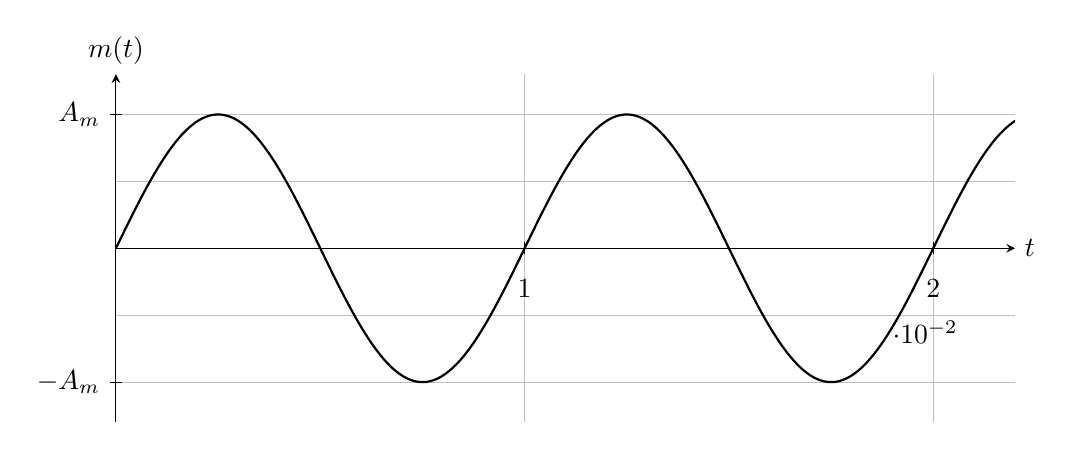
\begin{tikzpicture}
  \begin{axis}[
        height=6cm,
        width=13cm,
        axis lines=middle,
        grid=both,
        domain={0:0.03},
        ymin=-1.3, ymax=1.3,
        xmin=0, xmax=0.022,
        major tick length=1ex,
        minor tick length=0pt,
        tick style={color=black,thin},
        xtick={0.01, 0.02},
        xticklabels={$1$, $2$},
        minor xtick={0,0.01,...,0.03},
        xlabel=$t$,
        every axis x label/.style={
            at={(ticklabel* cs:1)},
            anchor=west,
        },
        xticklabel shift={.2cm},
        ytick={-1,1},
        yticklabels={$-A_m$, $A_m$},
        minor ytick={-0.5,0.5},
        ylabel=$m(t)$,
        every axis y label/.style={
            at={(ticklabel* cs:1)},
            anchor=south,
        },
        ]
    % \addplot[thin, dashed] coordinates { (80, 0) (80, 0.642788) (0, 0.642788) };
    % \draw[thick,blue] plot[domain=0:4.5,samples=200] (\t,{cos(deg(pi*\t))});
    \addplot[thick, black, samples=1000] { sin(deg(2*pi*100*x)) };
    % \addplot+[mark=*, color=black, mark options={scale=0.75,fill=black}] coordinates { (80, 0.642788) };
    % \node at (axis cs:0,0.642788) [anchor=east] {$\sigma_v$};
    % \node at (axis cs:80,0) [anchor=north] {$\sigma_\phi$};
    \end{axis}
\end{tikzpicture}
\end{center}

In de figuur is de tijdsas niet op schaal getekend, omdat een golf van $440$ Hz zo snel op en neer beweegt dat het op de figuur niet zichtbaar zou zijn.

Ik zou kunnen proberen dit geluid zoals het is door te sturen. Maar geluid draagt niet z\'o heel ver. Daarom plaatsen we de informatie op een draaggolf. Dit is een hoogfrequente sinuso\"idale EM golf met frequentie $fd$ in het $MHz-GHz$ gebied. Dit is een radiogolf. De draaggolf heeft als functievoorschrift $d(t) = A_d ~\sin (2 \pi f_d t)$. Hieronder zie je een voorbeeld van zo'n draaggolf $d(t)$:

\begin{center}
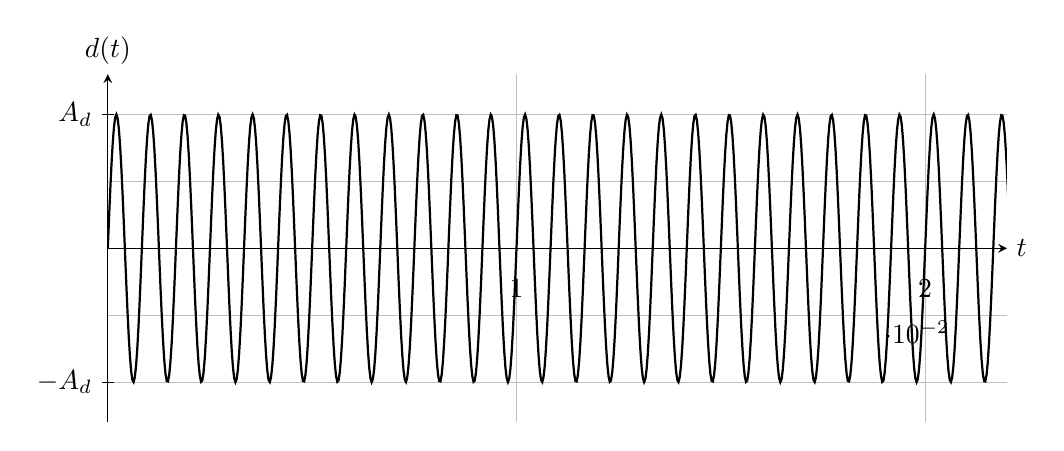
\begin{tikzpicture}
  \begin{axis}[
        height=6cm,
        width=13cm,
        axis lines=middle,
        grid=both,
        domain={0:0.03},
        ymin=-1.3, ymax=1.3,
        xmin=0, xmax=0.022,
        major tick length=1ex,
        minor tick length=0pt,
        tick style={color=black,thin},
        xtick={0.01, 0.02},
        xticklabels={$1$, $2$},
        minor xtick={0,0.01,...,0.03},
        xlabel=$t$,
        every axis x label/.style={
            at={(ticklabel* cs:1)},
            anchor=west,
        },
        xticklabel shift={.2cm},
        ytick={-1,1},
        yticklabels={$-A_d$, $A_d$},
        minor ytick={-0.5,0.5},
        ylabel=$d(t)$,
        every axis y label/.style={
            at={(ticklabel* cs:1)},
            anchor=south,
        },
        ]
    % \addplot[thin, dashed] coordinates { (80, 0) (80, 0.642788) (0, 0.642788) };
    % \draw[thick,blue] plot[domain=0:4.5,samples=200] (\t,{cos(deg(pi*\t))});
    \addplot[thick, black, samples=1000] { sin(deg(2*pi*1200*x)) };
    % \addplot+[mark=*, color=black, mark options={scale=0.75,fill=black}] coordinates { (80, 0.642788) };
    % \node at (axis cs:0,0.642788) [anchor=east] {$\sigma_v$};
    % \node at (axis cs:80,0) [anchor=north] {$\sigma_\phi$};
    \end{axis}
\end{tikzpicture}
\end{center}

Opnieuw is de tijdsas niet op schaal getekend, omdat een golf met frequenties in de grootteorde van $MHz$ zo snel op en neer beweegt dat het op de figuur niet zichtbaar zou zijn.

We laten de amplitude van de draaggolf vari\"eren naargelang de amplitude van het informatiesignaal. Dit doen we door beide golven te vermenigvuldigen als volgt:

\begin{eqnarray*}
    r(t) &=& (1 + \frac{1}{A_d} m(t)) \cdot d(t) \\
    &=& \left( 1 + \frac{1}{A_d} A_m \sin(2 \pi f_m t) \right) \cdot A_d \sin(2 \pi f_d t) \\
    &=& A_d \sin(2 \pi f_d t) + \frac{A_m}{A_d} A_d \sin(2 \pi f_m t) \sin(2 \pi f_d t) \\
    &=& A_d \sin(2 \pi f_d t) + m A_d \sin(2 \pi f_m t) \sin(2 \pi f_d t) \\
    &=& A_d \sin(2 \pi f_d t) + \frac{m A_d}{2} \cos(2 \pi (f_c+f_m) t) - \frac{m A_d}{2} \cos(2 \pi (f_c-f_m) t)  \\
\end{eqnarray*}

De factor $m$ die in de vergelijkingen hierboven verschijnt, is gedefinieerd als de verhouding van de amplitude van het modulatiesignaal tot de amplitude van de draaggolf, $\frac{A_m}{A_d}$. Dit noemen we de modulatiediepte. Het is een parameter die aangeeft hoe sterkt de amplitude van de gemoduleerde golf varieert in functie van de amplitude van het modulatiesignaal. $m$ varieert typisch tussen 0 (geen amplitudevariatie) tot 1 (sterke amplitudevariatie).

Het bekomen signaal $r(t)$ ziet er dan als volgt uit:

\begin{center}
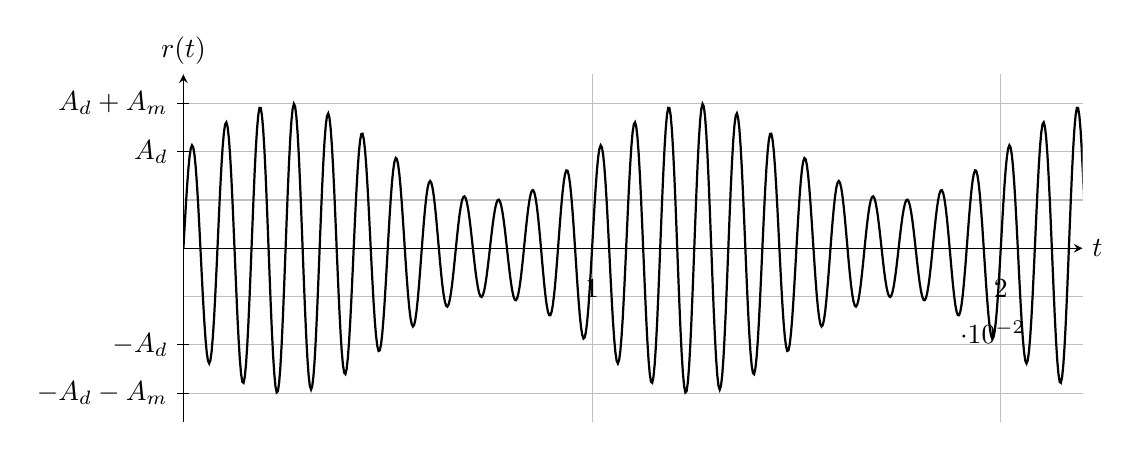
\begin{tikzpicture}
  \begin{axis}[
        height=6cm,
        width=13cm,
        axis lines=middle,
        grid=both,
        domain={0:0.03},
        ymin=-1.8, ymax=1.8,
        xmin=0, xmax=0.022,
        major tick length=1ex,
        minor tick length=0pt,
        tick style={color=black,thin},
        xtick={0.01, 0.02},
        xticklabels={$1$, $2$},
        minor xtick={0,0.01,...,0.03},
        xlabel=$t$,
        every axis x label/.style={
            at={(ticklabel* cs:1)},
            anchor=west,
        },
        xticklabel shift={.2cm},
        ytick={-1,-1.5,1,1.5},
        yticklabels={$-A_d$,$-A_d-A_m$,$A_d$,$A_d+A_m$},
        minor ytick={-1.5,-0.5,0.5,1.5},
        ylabel=$r(t)$,
        every axis y label/.style={
            at={(ticklabel* cs:1)},
            anchor=south,
        },
        ]
    % \addplot[thin, dashed] coordinates { (80, 0) (80, 0.642788) (0, 0.642788) };
    % \draw[thick,blue] plot[domain=0:4.5,samples=200] (\t,{cos(deg(pi*\t))});
    \addplot[thick, black, samples=1000] {(1+ 0.5*sin(deg(2*pi*100*x)))* sin(deg(2*pi*1200*x))  };
    % \addplot+[mark=*, color=black, mark options={scale=0.75,fill=black}] coordinates { (80, 0.642788) };
    % \node at (axis cs:0,0.642788) [anchor=east] {$\sigma_v$};
    % \node at (axis cs:80,0) [anchor=north] {$\sigma_\phi$};
    \end{axis}
\end{tikzpicture}
\end{center}

Het bekomen signaal $r(t)$ wordt dan via een antenne uitgestuurd. Je ziet dat het signaal alle informatie van $i(t)$ bevat: het signaal volgt de amplitudevariaties in $i(t)$. Bovendien draagt het signaal $r(t)$ verder dan het oorspronkelijke signaal $i(t)$ doordat het een EM golf met een hoge frequentie is.

In dit voorbeeld werd ge\"illustreerd hoe een sinuso\"idaal informatiesignaal kan gebruikt worden om een draaggolf te moduleren. Dit resulteerde in drie sinuso\"idale signalen: eentje met amplitude $A_d$ op de draaggolffrequentie $f_d$, eentje met amplitude $\frac{mA_d}{2}$ in de lage zijband op frequentie $f_d-f_m$ en eentje met amplitude $\frac{mA_d}{2}$ in de hoge zijband op frequentie $f_d+f_m$.

In de realiteit worden meer complexe informatiesignalen gebruikt om de draaggolf te moduleren. Dat kan bv. een spraaksignaal zijn. Hieronder zie je een voorbeeld:

% \begin{center}
% \begin{tikzpicture}[
%     declare function={
%       excitation(\t,\w) = sin(\t*\w);
%       noise = rnd - 0.5;
%       source(\t) = excitation(\t,20) + noise;
%       filter(\t) = 1 - abs(sin(mod(\t, 50)));
%       speech(\t) = 1 + source(\t)*filter(\t);
%     }
%   ]
%   \begin{axis}[
%         height=6cm,
%         width=13cm,
%         axis lines=middle,
%         grid=both,
%         domain={0:0.03},
%         ymin=-1.8, ymax=1.8,
%         xmin=0, xmax=0.022,
%         major tick length=1ex,
%         minor tick length=0pt,
%         tick style={color=black,thin},
%         xtick={0.01, 0.02},
%         xticklabels={$1$, $2$},
%         minor xtick={0,0.01,...,0.03},
%         xlabel=$t$,
%         every axis x label/.style={
%             at={(ticklabel* cs:1)},
%             anchor=west,
%         },
%         xticklabel shift={.2cm},
%         ytick={-1,-1.5,1,1.5},
%         yticklabels={$-A_d$,$-A_d-A_m$,$A_d$,$A_d+A_m$},
%         minor ytick={-1.5,-0.5,0.5,1.5},
%         ylabel=$A$,
%         every axis y label/.style={
%             at={(ticklabel* cs:1)},
%             anchor=south,
%         },
%         ]
%     % \addplot[thin, dashed] coordinates { (80, 0) (80, 0.642788) (0, 0.642788) };
%     % \draw[thick,blue] plot[domain=0:4.5,samples=200] (\t,{cos(deg(pi*\t))});
%     \addplot[thick, black, samples=1000] {\x,speech(\x)}
%     % \addplot[thick, black, samples=1000] {(1+ 0.5*sin(deg(2*pi*100*x)))* sin(deg(2*pi*1200*x))  };
%     % \addplot+[mark=*, color=black, mark options={scale=0.75,fill=black}] coordinates { (80, 0.642788) };
%     % \node at (axis cs:0,0.642788) [anchor=east] {$\sigma_v$};
%     % \node at (axis cs:80,0) [anchor=north] {$\sigma_\phi$};
%     \end{axis}
% \end{tikzpicture}
% \end{center}

% \begin{center}
%     \begin{tikzpicture}[
%     x=0.0085cm, y=0.5cm,
%     declare function={
%       excitation(\t,\w) = sin(\t*\w);
%       noise = rnd - 0.5;
%       source(\t) = excitation(\t,20) + noise;
%       filter(\t) = 1 - abs(sin(mod(\t, 50)));
%       speech(\t) = 1 + source(\t)*filter(\t);
%       sinewave(\t) = sin(2*pi*100*\t);
%                     },
%     orange, thick, smooth,          % <--- moved here
%     domain=0:360, samples=144,      % <--- moved here
%   ]
%     \draw plot (\x,{6+speech(\x)}); % <---
%     \draw plot (\x,{3+speech(\x)}); % <---
%     \draw plot (\x,{0+speech(\x)}); % <---
%     %
%     \draw[black, densely dotted, very thick]   (0,2.2) -- (0,2.8)
%                                         (0,5.2) -- (0,5.8);
%      \end{tikzpicture}
% \end{center}
\todo{Figuur voor spraak afwerken!}
% \begin{center}
%     \begin{tikzpicture}[
%     declare function={
%       excitation(\t,\w) = sin(\t*\w);
%       noise = rnd - 0.5;
%       source(\t) = excitation(\t,10) + noise;
%       filter(\t) = 1 - abs(sin(mod(\t, 10)));
%       speech(\t) = 1 + source(\t)*filter(\t);
%                     },
%   ]
% \begin{axis}[samples=500,domain=0:0.02,restrict y to domain =-20:100]
% \addplot[black]plot (\x, {6+speech(\x)});
% \addplot[black]plot (\x, {4+sin(deg(2*pi*1000*\x ))});
% \addplot[black]plot (\x, {(1+speech(\x))*sin(deg(2*pi*1000*\x ))});
% \end{axis}
% \begin{axis}[samples=500,domain=-6*pi:6*pi,restrict y to domain =-20:100]
% \addplot[very thick,yellow ]plot (\x, {sin((2*\pi*10*\x )});
% \end{axis}
% \begin{axis}[samples=500,domain=-6*pi:6*pi,restrict y to domain =-20:100]
% \addplot[very thick,yellow ]plot (\x, {sin((2*\pi*10*\x )});
% \end{axis}
% \end{tikzpicture}
% \end{center}

Modulatie met complexere informatiesignalen resulteert ook in een meer complex frequentiespectrum, met bijdragen op allerlei frequenties rond de draaggolffrequentie.

\subsubsection{Frequentie-modulatie (FM)}

Bij amplitude-modulatie volgt de amplitude van het gemoduleerde signaal het modulatiesignaal. De nuttige informatie zit dus in de amplitude! Dit betekent dat het ontvangen signaal erg verstoord zal zijn als er veel ruis op de verbinding zit: ruis zorgt er immers voor dat de amplitude van het ontvangen signaal afwijkt van de amplitude van het verzonden signaal. Deze ruis is moeilijk te verwijderen!

Een alternatieve modulatietechniek is frequentie-modulatie (FM). Bij FM zit de nuttige informatie in de frequentie van het gemoduleerde signaal. Bij AM zit de nuttige informatie in de amplitude van het gemoduleerde signaal.

Hieronder zie je een voorbeeld:

\begin{center}
	\tikzsetfigurename{module3_fig_FM}
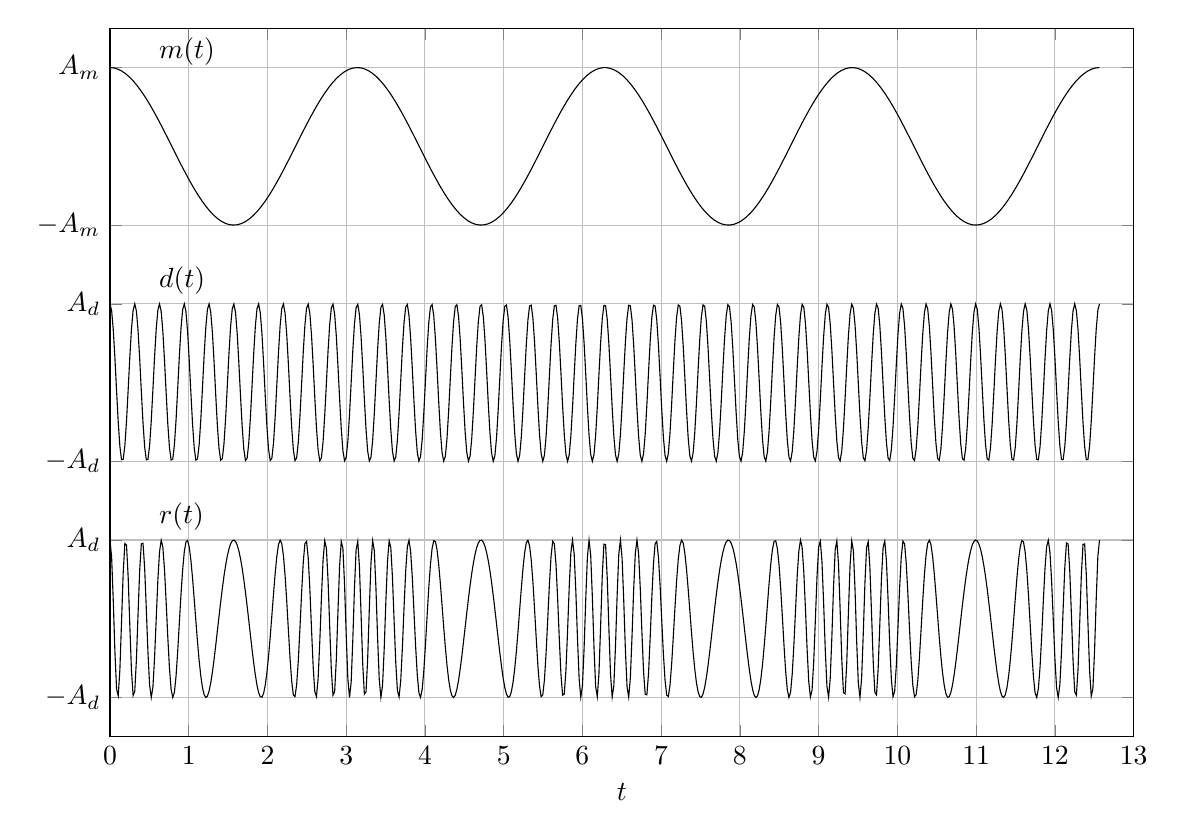
\begin{tikzpicture}
    \begin{axis}[
        grid=both,
        x=1cm,y=1cm,
        ymin = -7.5, ymax=1.5,
        xmin = 0, xmax = 13,
        xlabel = $t$,
        ytick={-1,1,-4,-2,-7,-5},
        yticklabels={$-A_m$, $A_m$,$-A_d$,$A_d$,$-A_d$,$A_d$}
    ]
      \addplot[domain=0:4*pi,black,samples=250] {cos(x*2*180/pi)};
        \addplot[domain=0:4*pi,black,samples=600] {cos(x*20*180/pi)-3};
      \addplot[domain=0:4*pi,black,samples=600] {cos((x*20 + 6*sin(x*2*180/pi))*180/pi)-6};
      
      \node[above,right] at (0.5,1.2) {$m(t)$};
      \node[above,right] at (0.5,-1.7) {$d(t)$};
      \node[above,right] at (0.5,-4.7) {$r(t)$};
    \end{axis}
\end{tikzpicture}
\end{center}

In het frequentie-gemoduleerde signaal $r(t)$ varieert de frequentie met de amplitude van het modulatiesignaal $m(t)$: 

\begin{itemize}
    \item wanneer de amplitude van $m(t)$ groot is, is de frequentie van $r(t)$ hoger
    \item wanneer de amplitude van $m(t)$ klein (negatief) is, is de frequentie van $r(t)$ lager
\end{itemize}

De concrete bewerking om het draaggolfsignaal te moduleren is frequentie-modulatie. De wiskunde is nogal ingewikkeld, dus die laten we hier achterwege.

% \subsection{Digitale modulatietechnieken}

% \subsubsection{On-off keying}

\mybox{
\subsection{Modulatietechnieken in IoT toepassingen}
Zoals gezegd gebruiken wij LoRa als de draadloze communicatietechnie. LoRa gebruikt een variant van frequentie-modulatie gebruikt. Er worden eigenlijk bits - eentjes en nulletjes - doorgestuurd. Bij een 1-bit is de draaggolf z\'o gemoduleerd dat de frequentie toeneemt. Bij de 0-bit is de draaggolf z\'o gemoduleerd dat de frequentie afneemt. Detectie of de frequentie toe- of afneemt, geeft dus rechtstreeks informatie over de verstuurde bit. 

\subsubsection{Digitale versus analoge communicatie}

Hier hebben we het over versturen van bits; we noemen dit digitale communicatie. Het alternatief is analoge commmunicatie. Met analoog bedoelen we een signaal dat continu is in de tijd en in amplitude. Zoals je in de voorbeelden van de analoge modulatietechnieken AM en FM kan zien, is het modulatiesignaal continu: het heeft een waarde op elk tijdstip. Bovendien kunnen alle amplitudes tussen twee grenzen voorkomen. 

Om een analoog signaal te digitaliseren, worden twee operaties uitgevoerd:
\begin{itemize}
    \item Het analoog signaal wordt eerst gediscretiseerd: de meetwaarden zijn slechts op bepaalde tijdstippen bepaald. 
	
    Naast \emph{discrete} signalen (in de figuur hieronder in rood aangeduid) bestaan ook \emph{continue} signalen (in de figuur hieronder in zwart aangeduid), waarvoor op elk moment een meetwaarde beschikbaar is. Het signaal loopt dus - zoals de naam het zegt - continu door.
	
    \gewonefiguur{width=\linewidth}{module3/discreetvscontinu}
    
    \item Vervolgens wordt het signaal in amplitude gedigitaliseerd: slechts een beperkt aantal amplitudes wordt behouden. Die amplitudes kunnen dan als een binair getal - in bits - uitgedrukt worden. Bij digitale communicatie worden die bits uiteindelijk verstuurd.
    
    In de figuur hieronder zie je links en rechts hetzelfde analoge signaal (in zwart) dat gedigitaliseerd werd: het is gekend op discrete tijdsstippen en slechts een beperkt aantal amplitudes is mogelijk. In de linkse figuur werd een ruwe selectie van amplitudes gemaakt: de fout tussen de amplitude van het analoge en het digitale signaal is redelijk groot. In de rechtse figuur werd een fijnere amplitudeverdeling gebruikt, waardoor het verschil tussen de amplitude van het analoge en het digitale signaal ook kleiner is.
    
    \gewonefiguur{width=\linewidth}{module3/analoogvsdigitaalAmplitude}
\end{itemize}

Versturen van bits (dit is digitale informatie!) zorgt ervoor dat de communicatie minder ruisgevoelig is, dan wanneer het modulatiesignaal analoog doorgestuurd wordt. Er kunnen immers minder fouten gemaakt worden wanneer enkel een 0- of 1-bit moet herkend worden dan wanneer de amplitude exact moet gereconstrueerd worden.
}

\subsection{Extra bewerkingen}

Naast de modulatie van de signalen, kunnen er in de zender nog een aantal extra bewerkingen uitgevoerd worden:
\begin{itemize}
    \item De \emph{broncodering} tracht zo goed mogelijk de redundantie die aanwezig is in het signaal, te verwijderen. Als resultaat hoopt men op een zo groot mogelijke compressie, waardoor de netto hoeveelheid door te sturen signalen geminimaliseerd wordt, en het transmissiekanaal efficiënt kan benut worden.
    \item Men kan de door te sturen informatie \emph{encrypteren} (ook wel \emph{vercijferen} genoemd), om ze te beveiligen tegen ongeoorloofd gebruik. Geheimhouding van informatie over draadloze verbindingen is een aspect waar men terecht nogal sceptisch tegenover staat, aangezien de signalen die door de lucht propageren in principe vrij beluisterd kunnen worden. Indien men echter gebruik maakt van de meest performante algoritmes die vandaag in de cryptografie voorhanden zijn, kan men draadloze verbindingen perfect beveiligen.
    \item De \emph{kanaalcodering} of \emph{foutcodering} gaat op een gecontroleerde manier extra informatie aan de signalen toevoegen, waaruit men na ontvangst eventuele problemen die opgetreden zijn tijdens de transmissie, hoopt te herstellen.
\end{itemize}

De basiselementen van een zender worden teruggevonden in om het even wel telecommunicatie-systeem en ze zijn dus niet eigen aan draadloze verbindingen, al zullen ze vaak wel specifieke implementaties kennen aangepast aan het transmissiekanaal.

In de ontvanger dienen de omgekeerde bewerkingen te gebeuren, om de informatie terug uit de doorgestuurde signalen te kunnen halen en deze aan de bestemming te kunnen afleveren. Dit betekent dat er eerst en vooral een demodulatie moet gebeuren, en vervolgens eventueel ook nog een kanaaldecodering en/of ontcijfering en/of brondecodering.

% \mybox{
% \subsection{Informatie-overdracht in IoTree}
% }

\section{Internet of Things: samenvatting}
\mybox{
\begin{itemize}
    \item In IoT toepassingen wordt informatie van sensoren (temperatuur en hellingsgraad, gemeten door een sensor) draadloos doorgestuurd naar een ontvangstantenne, de gateway genoemd.
    \item De gebruikte draadloze communicatietechniek onze IoT  toepassing is LoRa. 
    \item Bij de selectie van een communicatietechniek moet een afweging gemaakt worden tussen:
    \begin{itemize}
        \item Vermogenverbruik: hoeveel vermogen verbruikt je toepassing? Hoe meer energieverbruik, hoe sneller de batterij van je sensoren zal moeten vervangen worden.
        \item Communicatiebereik: wat is de maximale afstand tussen zender (sensor) en ontvanger (gateway) opdat er nog communicatie mogelijk is? Dit hangt af van de omgeving: reflecties, absorptie, diffractie, ... zorgen er immers voor dat het informatiesignaal verstoord bij de ontvanger aankomt! Ook de gekozen modulatietechniek bepaalt hoe robuust je communicatiesysteem is voor storende invloeden, zoals bv. ruis.
        \item Datasnelheid: hoeveel informatie kan je per tijdseenheid versturen? Als je continu video moest streamen, zal je een hogere datasnelheid nodig hebben, dan wanneer je elk kwartier de temperatuur van een boom wilt kennen.
        % \item Bandbreedte: 
    \end{itemize}
    Zoals in elk ontwerpprobleem moet ook bij de keuze van de draadloze communicatietechnologie een evenwicht gezocht worden tussen verschillende vereisten. “There is no such thing as free lunch”: je kan niet alles krijgen in het leven wat je zou willen. Binnen dit project werd gekozen voor de communicatietechnologie LoRa (Long Range). 
    
    We lijsten hieronder de voor- en nadelen van LoRa-communicatie op:
    \begin{itemize}
        \item[+] energiezuinig: de draadloze communicatie kost niet veel energie, waardoor de sensormodules lang op eenzelfde batterij kunnen functioneren zonder dat de batterij moet vervangen worden. Bij optimale condities zou een batterijduur langer dan jaar geen uitzondering zijn.
        \item[+] groot draadloos bereik: de sensoren kunnen tot op grote afstand gegevens naar de gateway doorsturen. In sommige gevallen tot wel 40 km ver! In praktische omstandigheden kan je berichten sturen tot wel enkele kilometers ver.
        \item[-] Beperkte hoeveelheid data die kan doorgestuurd worden binnen een vast tijdsinterval. Daardoor is het niet mogelijk geluid of video continu door te sturen. Afhankelijk van het aantal en type sensoren kunnen sensormodules ongeveer om de 5 minuten de sensorwaarden doorsturen.
    \end{itemize}
    \item Bij LoRa wordt een vorm van frequentiemodulatie (FM) gebruikt.
    %TODO iets over encryptie
    \item LoRa gebruikt ook foutcodering om fout gedetecteerde bits op te sporen en eventueel te corrigeren.
\end{itemize}
}



